\documentclass[12pt]{article}
\usepackage[margin=1in]{geometry} 
\usepackage{amsmath,amsthm,amssymb,amsfonts}
\usepackage{mathrsfs}
\usepackage{manfnt}
\usepackage{bbm}
\usepackage[shortlabels]{enumitem}
\usepackage{float}
%%% This is for drawing with tikz
\usepackage{tikz}
\usetikzlibrary{positioning,chains,fit,shapes,calc,arrows,patterns,cd,knots,hobby} 
\usepackage{tkz-graph}
\usetikzlibrary{arrows, petri, topaths}
\usepackage{tkz-berge}
\usepackage[all]{xy}
\usepackage{titling}
\usepackage{graphicx}
\usepackage{graphics}
\usepackage{float}
\usepackage{fancyhdr}

% Additional packages (included by Eappen)
\usepackage{fullpage}	% To use more of the page
\usepackage{times}		% To use Times New Roman instead of Computer Modern
\usepackage{mathtools}
\usepackage{epstopdf}
\usepackage{subcaption}

% To create new paragraphs
\setlength{\parindent}{0em}
\setlength{\parskip}{1em}

\DeclarePairedDelimiter{\abs}{\lvert}{\rvert}

\newcommand{\reals}{\mathbb R}

% To do a raised plus/minus symbol
\newcommand{\rpm}{\raisebox{.2ex}{$\scriptstyle\pm$}}

\renewcommand\maketitlehooka{\null\mbox{}\vfill}
\renewcommand\maketitlehookd{\vfill\null}

% For graphics / images
\usepackage{graphicx}
\setkeys{Gin}{width=\linewidth,totalheight=\textheight,keepaspectratio}
\graphicspath{{Graphics/}}

%augmented matrix:
\newenvironment{amatrix}[1]{%
	\left(\begin{array}{@{}*{#1}{c}|c@{}}
	}{%
	\end{array}\right)
}

%Math Shortcuts
\def \U {{\cal {U}}} 
\def \P {{\cal {P}}}
\def \Z {\mathbb{Z}}
\def \N {\mathbb{N}}
\def \Q {\mathbb{Q}}
\def \R {\mathbb{R}}
\def \C {\mathbb{C}}
\def \F {\mathbb{F}}
\def \ms {\medskip}
\def \ss {\smallskip}
\def \no {\noindent}
\def \vl {\overline}
\def \ub {\underline}
\def \cl {\centerline}
\def \dl {\displaystyle}
\def \lra {\longrightarrow}
\def \thus {{.\raise 4pt\hbox{.}.\;}}
\def \ctrdct {\rightarrow \!\leftarrow}
\def \div {{\bf {~div~}}}
\def\notdiv{\not|\;}
\font\Bigbf = cmr10 scaled\magstep 2
\font\sm = cmr10 scaled 900
\font\headerfont = cmti10 scaled 600
\def\LaTeX{{\rm L\kern-.36em\raise.3ex\hbox{\sc a}\kern-.15em\TeX}}

\def\doblue #1 {\color{blue}}
%%%% Shortcut Macros
\newcommand{\setcomplement}[1]{{#1}^{\mathsf{c}}}
\newcommand{\fl}{\flushright}

\newcommand{\bunderline}[1]{\underline{#1}}
\renewcommand{\vec}[1]{{\bunderline{#1}}}
\newcommand{\vect}[1]{{\bunderline{#1}}} 
\newcommand{\mat}[1]{{\bunderline{\bunderline{#1}}}}


%%% Problem environment
% \newcounter{ProblemNumber}
% \setcounter{ProblemNumber}{0}
% \newenvironment{problem}[1][Problem]{\begin{trivlist}
% \item[\hskip \labelsep {\bfseries #1}\hskip \labelsep \stepcounter{ProblemNumber}{\bfseries \arabic{ProblemNumber}.}]}{\end{trivlist}}

\newenvironment{problem}[2][Problem]{\begin{trivlist}
		\item[\hskip \labelsep {\bfseries #1}\hskip \labelsep {\bfseries #2.}]}{\end{trivlist}}
%If you want to title your bold things something different just make another thing exactly like this but replace "problem" with the name of the thing you want, like theorem or lemma or whatever
\newtheorem{theorem}{Theorem}

\newcommand{\solution}{\textit{Solution:}}
% Make proof environment look like amslatex's
%\renewcommand{\qedsymbol}{\square}% PLEASE NOTE: this is in the AMS symbols font.
%\makeatletter
%\renewenvironment{proof}[1][\proofname]{\par
%  \pushQED{$\qedsymbol$}%
%  \normalfont \topsep6\p@\@plus6\p@\relax
%  \list{}{\leftmargin=1.25mm\itemindent=20pt\linewidth=0.975\textwidth%
%  \item[\hskip\labelsep
%        \bfseries
%   #1\@addpunct{.}]\ignorespaces}
%}{%
%  \popQED\endlist\@endpefalse
%}



\begin{document}
%June 4
Suppose that the $xy$ coordinate system is the original coordinate system, and we have rotated the coordinate system by an angle $\omega$ to obtain the $sz$ coordinate system.
We can convert between the two coordinate systems using the following relationships:
\begin{align*}
	x(s, z; \omega) & = s \cos (\omega) - z \sin (\omega) \\
	y(s, z; \omega) & = s \sin(\omega) + z \cos (\omega)
\end{align*}
Once we pick $\omega$, we can measure $\hat{f}(s_{k}; \omega)$ for $k = 1, 2, 3, \hdots$ (for however many receiver locations there are).
We can then pick another $\omega$ and repeat the above process. 
\par 
Suppose $s$ is a continuous variable.
We denote $\hat{f}(s, \omega)$ to be the Radon transform of $f(x, y)$, and is defined by
\begin{align*}
	\hat{f}(s, \omega) & := \int_{-\infty}^{\infty} f(x, y) dz \\
					   & = \int_{-\infty}^{\infty} f\big( s \cos (\omega) - z \sin (\omega), s \sin(\omega) + z \cos (\omega) \big) dz
\end{align*}
where we have used the relationships between the $xy$ and $sz$ coordinate systems.
Note that the $z$ variable disappears because we are taking the line integral with respect to $z$ in the above definition. 
\par 
The \underline{imaging problem} (or inverse problem) is given $\hat{f}(s, \omega)$ (the Radon transform of $f(x, y)$), we want to recover $f(x, y)$.
\par 
Suppose we fix $\omega$.
Using the chain rule and the previous relationships between the $xy$ and $sz$ coordinate systems, we get that
\begin{align*}
	\frac{\partial}{\partial x} & = \frac{\partial s}{\partial x} \frac{\partial}{\partial s} + \frac{\partial z}{\partial x} \frac{\partial}{\partial z} \\
	\frac{\partial}{\partial y} & = \frac{\partial s}{\partial y} \frac{\partial}{\partial s} + \frac{\partial z}{\partial y} \frac{\partial}{\partial z}
\end{align*}
We can write the relationships between the $xy$ and $sz$ coordinate systems in matrix form:
\begin{align*}
	\begin{bmatrix}
		x \\
		y
	\end{bmatrix}
	& = 
	\begin{bmatrix}
		\cos (\omega) & - \sin (\omega) \\
		\sin (\omega) & \cos (\omega)
	\end{bmatrix}
	\begin{bmatrix}
		s \\
		z
	\end{bmatrix} \\
	& = C 
	\begin{bmatrix}
	s \\
	z
	\end{bmatrix}
\end{align*}
where $C = \begin{bmatrix} \cos (\omega) & - \sin (\omega) \\ \sin (\omega) & \cos (\omega)\end{bmatrix}$.
\par 
Multiplying the above equation on both sides by the inverse of $C$ (which we can easily verify is given by the following),
\begin{align*}
	C^{-1} & = 
	\begin{bmatrix}
		\cos (\omega)  & \sin(\omega) \\
		-\sin (\omega) & \cos(\omega)
	\end{bmatrix}
\end{align*}
we get that
\begin{align*}
	\begin{bmatrix}
	s \\
	z
	\end{bmatrix}
	& =
	\begin{bmatrix}
		\cos (\omega) & \sin (\omega) \\
		-\sin (\omega) & \cos (\omega)
	\end{bmatrix}
	\begin{bmatrix}
		x \\
		y
	\end{bmatrix}
\end{align*}
We see that
\begin{align*}
	\frac{\partial s}{\partial x} & = \cos (\omega) & \frac{\partial s}{\partial y} & = \sin (\omega) \\
	\frac{\partial z}{\partial x} & = -\sin (\omega) & \frac{\partial z}{\partial y} & = \cos (\omega)
\end{align*}
Thus
\begin{align*}
	\frac{\partial}{\partial x} & = \cos (\omega) \frac{\partial}{\partial s} -\sin (\omega) \frac{\partial}{\partial z} \\
	\frac{\partial}{\partial y} & = \sin (\omega) \frac{\partial}{\partial s} + \cos (\omega) \frac{\partial}{\partial z}
\end{align*}
We are interested in the Radon transform of $\frac{\partial f}{\partial x} := f_{, x}$.
By definition of the Radon transform from earlier, we have that $\widehat{f_{, x}}(s, w)$ (the Radon transform of $f_{, x}$) is defined as follows:
\begin{align*}
	\widehat{f_{, x}}(s, \omega) & = \int_{-\infty}^{\infty} f_{, x}(x, y) \, dz \\
							& = \int_{-\infty}^{\infty} f_{, x}(s \cos (\omega) - z \sin (\omega), s \sin (\omega) + z \cos (\omega)) \, dz \\
							& = \int_{-\infty}^{\infty} \Big( \cos (\omega) f_{, s} - \sin (\omega) f_{, z} \Big) \, dz \\
							& = \cos (\omega) \int_{-\infty}^{\infty} f_{, s} \, dz - \sin (\omega) \int_{-\infty}^{\infty} f_{, z} \, dz
\end{align*}
We can pull the partial derivative with respect to $s$ out of the first term in the above expression.
Furthermore, if we assume that $f$ has compact support, we get that $f(z = \infty) = 0$ and $f(z = -\infty) = 0$.
Thus,
\begin{align*}
	\int_{-\infty}^{\infty} \, f_{, z} dz & = f(z = \infty) - f(z = -\infty) \\
									   & = 0 - 0 \\
									   & = 0
\end{align*}
Thus, we get that
\begin{align*}
	\widehat{f_{, x}}(s, \omega) = \cos (\omega) \frac{\partial}{\partial s} \Bigg( \int_{-\infty}^{\infty} f \, dz \Bigg)
\end{align*}
From earlier, we know that $\hat{f}(s, \omega) = \int_{-\infty}^{\infty} f \, dz$, so we get that
\begin{align*}
	\widehat{f_{, x}}(s, \omega) & = \cos (\omega) \frac{\partial}{\partial s} \hat{f} (s, \omega) \\
								 & = \cos (\omega) \hat{f}_{, s} (s, \omega)
\end{align*}
where $\hat{f}_{, s} (s, \omega)$ denotes the partial derivative with respect to $s$ of the Radon transform of $f$.
In alternate notation,
\begin{align*}
	R(f_{, x}) (s, \omega) & = \cos (\omega) \frac{\partial}{\partial s} R(f) (s, \omega)
\end{align*}
We can compute the Radon transform of $\frac{\partial f}{\partial y} := f_{, y}$ in a similar manner.
\begin{align*}
	\widehat{f_{, y}}(s, \omega) & = \int_{-\infty}^{\infty} f_{, y} \, dz \\
								 & = \int_{-\infty}^{\infty} \Big( \sin(\omega) f_{, s} + \cos (\omega) f_{, z} \Big) \, dz \\
								 & = \sin (\omega) \frac{\partial}{\partial s} \int_{-\infty}^{\infty} f \, dz \\
								 & = \sin(\omega) \frac{\partial}{\partial s} \hat{f} (s, \omega) \\
								 & = \sin (\omega) \hat{f}_{, s} (s, \omega)
\end{align*}
In alternate notation,
\begin{align*}
	R(f_{, y}) (s, \omega) & = \sin (\omega) \frac{\partial}{\partial s} R(f) (s, \omega)
\end{align*}
We see that when we take Radon transforms of the partial derivatives of $f$, we end up dealing with only the partial derivatives of the Radon transform of $f$ with respect to $s$.

The current problem of interest is the solution to multi-dimensional (2D) partial differential equations of the form: $\vec{a}$

\begin{align}
	\vec{q}_{,t} + \mat{A} \, \vec{q}_{,x} + \mat{B}\, \vec{q}_{,y} = \vec{0} \label{eq1}
\end{align}

where $M$ is the number of equations in the system, and

\begin{align*}
	&\mat{A}, \mat{B} \in \R^{M \times M},\\
	&\vec{q}(t, \vec{x}) : \R^+ \times \R^2 \to \R^M.
\end{align*}

In particular, we are interested in the case of hyperbolic PDEs, for which the choice of $\mat{A}$ and $\mat{B}$ are limited.

Define $\mat{\widetilde{A}}(\alpha)$ such that

\begin{align*}
	\mat{\widetilde{A}}(\alpha) = \cos(\alpha)\mat{A} + \sin(\alpha)\mat{B}, \quad \alpha \in \R.
\end{align*}

Equation \ref{eq1} is hyperbolic if $\ub{\ub{\widetilde{A}}}(\alpha)$ is diagonalizable with only real eigenvalues for all $\alpha \in \R$.
That is to say, $\mat{\widetilde{A}}(\alpha) = \mat{R}\, \mat{\Lambda}\, \mat{R}^{-1}$ where $\mat{\Lambda} = \texttt{diag}(\lambda_1, \lambda_2, \dots, \lambda_M) \in \R^{M \times M}$ and the columns of $\mat{R}$ are linearly independent eigenvectors of $\mat{\widetilde{A}}(\alpha)$.

By this definition, systems with symmetric $\mat{\widetilde{A}}(\alpha)$ are among hyperbolic PDEs.
The hyperbolicity of a system relates to the transmission speed of information.
If the PDEs are hyperbolic, then the information is transmitted at a finite speed.
For example, the heat equations are not hyperbolic, while the wave equations are.

Combining the Randon Transform and hyperbolic PDEs: \\ 
We begin with our general form of the hyperbolic PDE which is a two-dimensional function with time
\begin{align*}
\vec{q}_{,t} + \mat{A}\,\vec{q}_{,x} + \mat{B}\,\vec{q}_{,y} = \vec{0}
\end{align*}
and then we begin to compute the Randon Transform on it. \\ 
Note: $q(t,x,y)$ will become $q(s,x)$ after the transformation. \\

\begin{align*}
R(\vec{q}_{,t}) = \frac{\partial}{\partial t} R(\vec{q}) \\
R(\mat{A}\,\vec{q}_{,x}) = \mat{A}R(\vec{q}_{,x}) = \mat{A}\cos(\omega)\frac{\partial}{\partial s}R(\vec{q}) \\
R(\mat{B}\,\vec{q}_{,y}) = \mat{B}R(\vec{q}_{,y}) = \mat{B}\sin(\omega)\frac{\partial}{\partial s}R(\vec{q}) \\
\end{align*}
We then combine these into the form:
\begin{align*}
\frac{\partial}{\partial t} R(\vec{q}) + \mat{A}\cos(\omega)\frac{\partial}{\partial s}R(\vec{q}) + \mat{B}\sin(\omega)\frac{\partial}{\partial s}R(\vec{q}) = \vec{0} \\
\widehat{\vec{q}}_{,t} + \widetilde{\mat{A}}(\omega)\widehat{\vec{q}}_{,s} = \vec{0} \\
\widetilde{\mat{A}}(\omega) = \cos(\omega)\mat{A} + \sin(\omega)\mat{B}
\end{align*}
The second equation is a collection of one-dimensional problems parameterized by $\omega$. \\

Initial Value Problems:
\begin{align*}
\vec{q}_{,t} + \mat{A}\,\vec{q}_{,x} + \mat{B}\,\vec{q}_{,y} = \vec{0} \\
q(t=0,x,y) = q_0(x,y)
\end{align*}

Process: \\
Step 1: Compute $R(q_0(x,y))$ \\
Step 2: Solve from $t=0$ to $t=T$
\begin{align*}
\widehat{\vec{q}}_{,t} + \widetilde{\mat{A}}(\omega)\widehat{\vec{q}}_{,s} = \vec{0} \\
\widehat{\vec{q}}(t=0,x,y) = R(q_0(x,y)
\end{align*}
Step 3: Compute $R^{-1}(\widehat{q}(T,s,w)$

%June 4
For right now, we will be setting the Radon Transform aside. \\

We need to work on solving:

\begin{align*}
\widehat{\vec{q}}_{,t} + \widetilde{\mat{A}}(\omega) \widehat{\vec{q}}_{,s} = \vec{0} \\
\widehat{\vec{q}}_{,t} + \widetilde{\mat{A}}\,\widehat{\vec{q}}_{,s} = \vec{0}
\end{align*}

We will be picking one value for $\omega$ so that we can figure out how to solve this first, therefore using the second equation. \\

There are two key ingredients to solving this: \\
1. We need to know how to discretize in time, which is sometimes called time-stepping. \\
2. We need to know how to discretize in "space" ("space" being our s variable)
We will be starting with discretizing "space".
In order to do this, we need to replace $\frac{\partial}{\partial s}$ by a discrete matrix $\mat{D}$ \\

An example of this is the Central Finite Differences for $\widehat{\vec{q}}_{,s}$: \\

\begin{align*}
\widehat{q}(s)\ms\lra\ms\widehat{\vec{Q}} =  [\,\widehat{q}(s_1)\ms,\ms\widehat{q}(s_2)\ms,\ms\widehat{q}(s_3)\ss.\ss.\ss.\ss]
\end{align*}

When working with a fixed time interval, we have a mesh with an even grid spacing.

\begin{figure}[H]
\centering
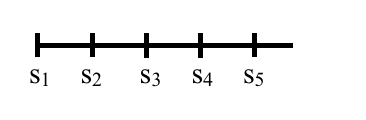
\includegraphics[width=0.25\textwidth]{MeshLine.jpg}
\caption{In the graphic above, the distance between the points is h units apart. This makes the graphic a uniform mesh.}
\end{figure}

To roughly discretize in space, we will use Central Finite Differences. 

\begin{align*}
\widehat{q}_{,s} |_{s_k} \approx \frac{\widehat{Q}_{k+1} - \widehat{Q}_{k-1}}{2h}
\end{align*}

This creates a 3-point stencil with error $O(h^2)$. 

\begin{align*}
\widehat{q}_{,s} \approx \mat{D}\,\widehat{\vec{Q}} = \frac{1}{2h}* \begin{bmatrix} 0&1&  &  &0 \\ -1&0&1  &  & \\   &-1&0&\ddots  &  \\   &  &\ddots&\ddots&1 \\ 0&  &  &-1&0 \end{bmatrix} \begin{bmatrix} \widehat{Q}_1 \\ \widehat{Q}_2 \\ \vdots \\ \widehat{Q}_{N-1} \\ \widehat{Q}_N \end{bmatrix}
\end{align*}
This however, is not exact. When we use a stencil in this manner, we end up with slight issues that relate to the boundary conditions. For now, we will ignore this fact and focus on the middle portion that includes the $-1, 0, 1$ signature. We can even create wider stencils, like a 5-point stencil, which has error $O(h^4)$.

When we use wider and wider stencils, we can theoretically produce more accurate approximations of the derivative:
\begin{align*}
\text{3-point stencil}\,\,\,\,\,\,\,\, \text{error}\,O(h^2) \\
\text{5-point stencil}\,\,\,\,\,\,\,\, \text{error}\,O(h^4) \\
\vdots\,\,\,\,\,\,\,\,\,\,\,\,\,\,\,\,\,\,\,\,\,\,\,\,\,\,\,\,\,\,\,\, \\
2k+1\text{-point stencil}\,\,\,\,\,\,\,\, \text{error}\,O(h^{2k})
\end{align*}
For generic $\widehat{q}(s)$, you don't observe optimal $O(h^{2k})$ accuracy. In fact, $|| \,\mat{D}\,\widehat{\vec{Q}} - \widehat{q}_{,s}\, || \lra \infty$ as $h \lra 0$. This is called the Runge phenomenon. \\
The problem is that we used equally spaced points. 
"Optimal" points that would work better for what we need would be Chebychev points. 
\begin{align*}
s \in [-1,1] \\
s_j = \cos(j\pi/N) \\
N+1 \,\, points \\
j = 0, 1, 2, . . .  \\
s_0 = 1 \,\,\,\,
s_N = -1
\end{align*}
\begin{figure}[H]
\centering
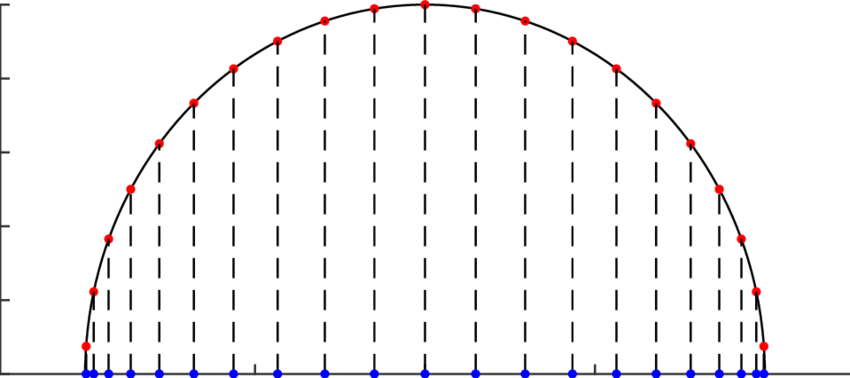
\includegraphics[width=0.8\textwidth]{ChebyshevPoints.jpg}
\caption{The above graphic has red dots to show the uniformly spaced points on the sine curve and blue dots to show the non-uniformly spaced Chebyshev points that will be used for our mesh.}
\end{figure}
The density of the grid points is high at the ends and low in the middle. Therefore, now we have a non-uniform mesh that has small spacing near $s = \rpm\,1$ and has large spacing near $s = 0$.\\
When we calculate the derivative at all points we get the following matrix. \\
\begin{figure}[H]
\centering
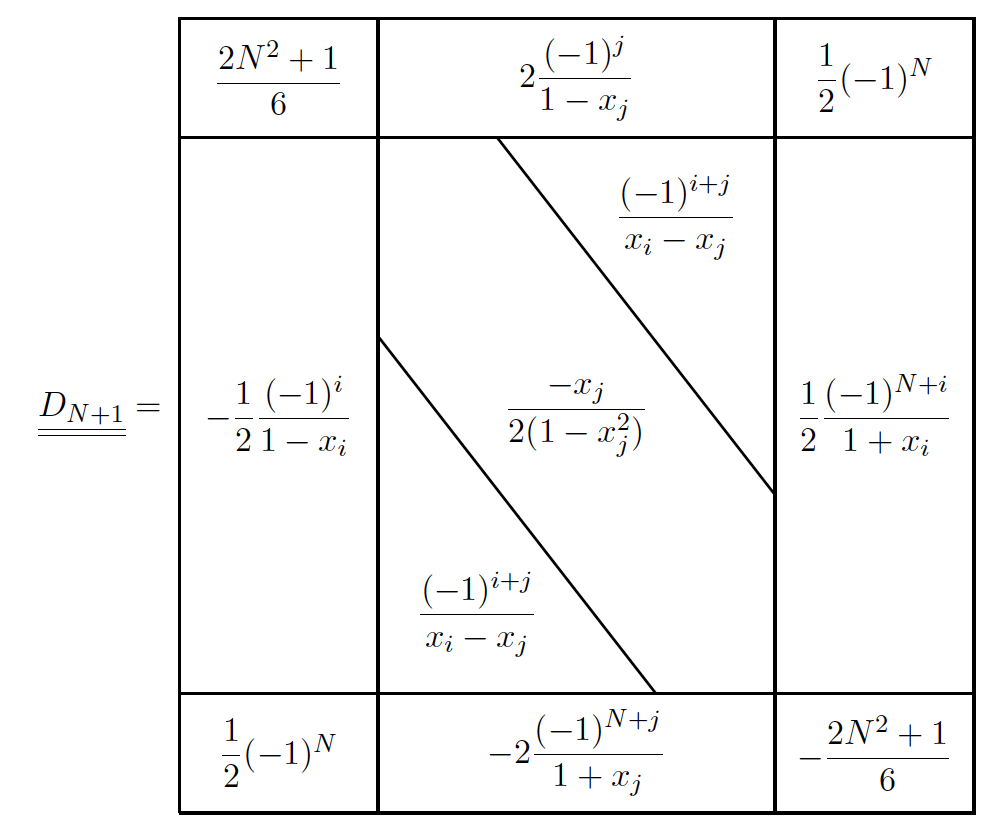
\includegraphics[width=0.8\textwidth]{Chebyshev.jpg}
\caption{This graph is from Spectral Methods in MATLab by Trefethen.}
\end{figure}
This is the Spectral Method. 

Today we wrote the code \texttt{spec\_diff.py}, a module that contains the function \texttt{spectral\_diff}.
This module takes as input a number of discretization points in space, optimized to be Chebyshev points, and optionally the range of those points. 
It returns the location of the discretization points, as well as the associated spectral differentiation matrix.
Its declaration and use is as follows:
$$\texttt{s, D\_N = spectral\_diff( N, a = -1, b = 1)}$$

This module is implemented through heavy use of numpy array indexing and broadcasting. 
This is done in an effort to limit the number of for-loops required, as the current code has none.
The diagonal of the matrix is constructed according to the numerically stable method described in Trefethen.
This method takes advantage of the fact that the sum of the columns in each row is 0.

Additionally, we begun work in the module \texttt{beuler\_advection.py}, which in its present state contains code to solve the following advection equation:
\begin{align*}
	&\hat{q}_{,t} + \hat{q}_{,s} = 0\\
	&\hat{q}(t=0, s) = \hat{q}_0(s) \quad s \in [-1, 1]
\end{align*}
The equation is discretized in space according to the above spectral method code, and is discretized in time with Backwards Euler. 
Presently, the code is incomplete, as solutions blow up near the edges of the domain.
It is suspected that the source of the error is mathematical, rather than programmatic. 

\subsection*{Time-stepping}
To explore time-stepping, we consider the advection equation:
\begin{align*}
	\hat{q}_{, t}(t, s) + \hat{q}_{, s}(s, t) & = 0, \, s \in [-1, 1] \\
	\hat{q}(t = 0, s) & = \hat{q}_{0}(s)
\end{align*}
If we discretize in space using the Chebyshev points (i.e. we consider the function values at the Chebyshev points on the interval $[-1, 1]$), we can use previous results to write that
\begin{align*}
	\hat{\vec{q}}_{, s} & \approx \mat{D_{N}} \, \hat{\vec{Q}}
\end{align*}
where $\mat{D_{N}}$ is the Chebyshev differentiation matrix corresponding to $(N + 1)$ Chebyshev points on the interval $[-1, 1]$ and $\hat{\vec{Q}}$ is the $(N+1) \times 1$ vector containing the approximate solution at the $(N + 1)$ Chebyshev points on the interval $[-1, 1]$.
\par 
Using the approximation to the partial derivative with respect to space, we are to able to obtain the semi-discrete form of the above PDE
\begin{align*}
	\frac{\partial}{\partial t} \hat{\vec{Q}} + \mat{D_{N}} \, \hat{\vec{Q}} & = \vec{0}
\end{align*}
which we can solve using the \underline{method of lines}.
\par 
To time-step, we can discretize the partial derivative with respect to time to obtain the fully discretized form of the PDE and pick a time-stepping method.
For example, we can use the \underline{forward Euler} method to time-step.
Forward Euler discretizes the partial derivative with respect to time in the following manner:
\begin{align*}
	\frac{\hat{\vec{Q}}^{n+1} - \hat{\vec{Q}}^{n}}{\triangle t} + \mat{D_{N}} \, \hat{\vec{Q}}^{n} & = \vec{0}
\end{align*}
where $\hat{\vec{Q}}^{n+1}$ is the approximate solution at the $(n+1)^{th}$ time step,  $\hat{\vec{Q}}^{n+1}$ is the approximate solution at the $n^{th}$ time-step, and $\triangle t$ is the time-step size. The forward Euler method can be easily derived.
\par 
We can rearrange the above equation as follows:
\begin{align*}
	\hat{\vec{Q}}^{n+1} & = \hat{\vec{Q}}^{n} - \triangle t \mat{D_{N}} \, \hat{\vec{Q}}^{n} \\
						& = \Big( \mat{I} - \triangle t  \mat{D_{N}} \Big) \hat{\vec{Q}}^{n}
\end{align*}
which allows us to compute the approximate solution at the Chebyshev points at the next time-step using the approximate solution at the current time-step.
Note that forward Euler is an \underline{explicit method}, and there is a dependence between the spatial and time-step size. 
If the time-step size is too large, as we compute the approximate solutions at successive time steps, the solutions will display numerical instability. 
We can use more stable explicit methods, such as the \underline{Runge-Kutta fourth order} method, but we still have to pay attention to the spatial and time step sizes.
\par 
We can also use \underline{implicit methods} to time-step.
The simplest implicit method is \underline{backward Euler}, and it discretizes the partial derivative with respect to time in the following manner:
\begin{align*}
	\frac{\hat{\vec{Q}}^{n+1} - \hat{\vec{Q}}^{n}}{\triangle t} + \mat{D_{N}} \, \hat{\vec{Q}}^{n+1} & = \vec{0}
\end{align*}
We can derive the backward Euler method by noting that we can put the PDE into the form
\begin{align*}
	\hat{q}_{, t}(t, s) & = -\hat{q}_{, s}(t, s)
\end{align*}
Since the above equation must hold for all time $t > t_{0}$ (where $t_0$ is the initial time), it must hold at the $(n+1)^{th}$ time step (denoted $t_{n+1}$).
We can use a backward difference approximation to approximate $\underline{\hat{q}}_{, t}$ at $t_{n+1}$, i.e.
\begin{align*}
	\vec{\hat{q}}_{, t}^{n+1} & \approx \frac{\hat{\vec{Q}}^{n+1} - \hat{\vec{Q}}^{n}}{\triangle t}
\end{align*}
and from previous results, we can approximate the partial derivative of $\hat{q}$ using the Chebyshev differentiation matrix i.e.
\begin{align*}
	\vec{\hat{q}}_{, s}^{n+1} & \approx \mat{D_{N}} \, \vec{\hat{Q}}^{n+1} 
\end{align*}
Substituting these approximations into the PDE, we get
\begin{align*}
	\frac{\hat{\vec{Q}}^{n+1} - \hat{\vec{Q}}^{n}}{\triangle t} & = -\mat{D_{N}} \, \vec{\hat{Q}}^{n+1} 
\end{align*}
After moving like terms to one side, we get
\begin{align*}
	\hat{\vec{Q}}^{n} & = \hat{\vec{Q}}^{n+1} + \triangle t \, \mat{D_{N}} \, \vec{\hat{Q}}^{n+1} \\
					  & = \Big( \mat{I} +  \triangle t \, \mat{D_{N}} \Big) \hat{\vec{Q}}^{n+1}
\end{align*}
We multiply the above equation by the inverse of the matrix (assuming the matrix is non-singular) on the right side to obtain
\begin{align*}
	\hat{\vec{Q}}^{n+1} & = \Big( \mat{I} +  \triangle t \, \mat{D_{N}} \Big)^{-1} \hat{\vec{Q}}^{n}
\end{align*}

%June 5
We want to find a higher order implicit method. So, for the moment, imaging that we are solving an ODE in time. 

\begin{align*}
\vec{q}' = \mat{A}\,\vec{q}
\end{align*}

A solution to this is the Taylor Series in time. To start, we will look at the explicit method.


\begin{align*}
\vec{q}(t + \Delta t) = \vec{q}(t) + \Delta t \vec{q}_{,t}(t) + &\frac{1}{2}\Delta t^2 \vec{q}_{,t,t}(t) + \frac{1}{6}\Delta t^3 \vec{q}_{,t,t,t}(t) + \dots \\
\vec{q}_{,t} &= \mat{A}\,\vec{q}  \\
\vec{q}_{,t,t} = \mat{A}\,&\vec{q}_{,t} = \mat{A}^2\,\vec{q} \\
\vdots& \\
\vec{q}_{,t,t,...,t} &= \mat{A}^n\,\vec{q}  \\
\therefore \vec{Q}^{n+1} = (\mat{I} + \Delta t \mat{A} + &\frac{1}{2} \Delta t^2\mat{A}^2 + \frac{1}{6}\Delta t^3 \mat{A}^3 + \dots)\vec{Q}^n
\end{align*}

The first two terms of the bottom equation make up the forward Euler method discussed earlier. These two terms are first order accurate, $O(\Delta t)$. The first three terms are second order accurate, $O(\Delta t^2)$. The first four terms are third order accurate, $O(\Delta t^3)$, and so on. These are all explicit methods. If we were to use this method, we would end up having to restrict our time step to a small window.  \\

Now, we will look at the implicit method.

\begin{align*}
\vec{q}(t) = \vec{q}(t + \Delta t) - \Delta t \vec{q}_{,t}(t + \Delta t) + &\frac{1}{2} \Delta t^2 \vec{Q}_{,t,t}(t + \Delta t) - \frac{1}{6} \Delta t^3 \vec{q}_{,t,t,t}(t + \Delta t) + \dots \\
\vec{q}_{,t} &= \mat{A}\,\vec{q} \\
\vec{q}_{,t,t} = \mat{A}\,&\vec{q}_{,t} = \mat{A}^2\,\vec{q} \\
\vdots& \\
\vec{q}_{,t,t,...,t} &= \mat{A}^n\,\vec{q} \\
%\text{The three equations above are still true from the explicit method} \\
\vec{q}(t) = (1 - \Delta t \mat{A} + \frac{1}{2} \Delta t^2& \mat{A}^2 - \frac{1}{6} \Delta t^3 \mat{A}^3 + \dots) \vec{q}(t + \Delta t) \\
\vec{Q}^{n+1} = [\mat{I} - \Delta t \mat{A} + &\frac{1}{2} \Delta t^2 \mat{A}^2 - \frac{1}{6} \Delta t^3 \mat{A}^3 + \dots]^{-1} \vec{Q}^n
\end{align*}

The first two terms of the bottom equation make up the backwards Euler method that was also discussed earlier. Like with the explicit method, the first two terms are first order accurate, the first three are second order accurate, and so on. In order to implement this, we don't need to change much of our code, we just need to change our formula.

As predicted yesterday, the errors in the spectral method are mathematical, not computational.
Specifically, this use of the spectral method does not account for the boundary conditions of the system.
Because the system has only advection to the right, the inflow of the equations is not accounted for, and was causing substantial numerical errors. 
5 solutions were proposed, each involved in ensuring that the solution at left-most chebyshev point remains zero throughout the advection.
\begin{enumerate}
	\item Set last row and last column of differentiation matrix to zero.
	\item Compute necessary powers of differentiation matrix, then set last row and last column to zero.
	Investigation has shown this to be equivalent to method 1.
	\item Removing the last row and column of differentiation matrix.
	\item Removing last row and column of the matrix operator applied to $\hat{\vec{Q}^n}$ at every timestep, either before or after inversion.
	\item Setting the last row of the above matrix to zero before or after inversion.
\end{enumerate}
The module $\texttt{beuler\_advection.py}$ contains the framework in which we are testing the above methods.
Additionally, the code has been refactored into the function $\texttt{advection}$ which has the following declaration:
$$\texttt{q, s = def advection( tf, N, dt, q0, domain=[-1, 1], ord=2, plot=True )}$$
where \texttt{tf} is the final time at which the solution is calculated, \texttt{N} is the number of spatial discretization points, \texttt{dt} is the time-step used, \texttt{q0} is a function representing the initial condition, and \texttt{ord} is the order used in the solution.
\texttt{q} is the solution at time \texttt{tf} located at each of the chebyshev points in \texttt{s}. 
Presently, only the order 1, 2, and 3 solutions are speculated to work, although this is not certain.
The reason for this uncertainty comes from uncertainty in the choice of solution to the boundary issue.
Among the above solutions, none works exactly for higher order methods, with coarser time discretization.
This is seen in the below figure, particularly for the 5-th order method.
The exact matrices used for the higher order implicit methods are discussed below.
\begin{figure}[H]
	\centering
	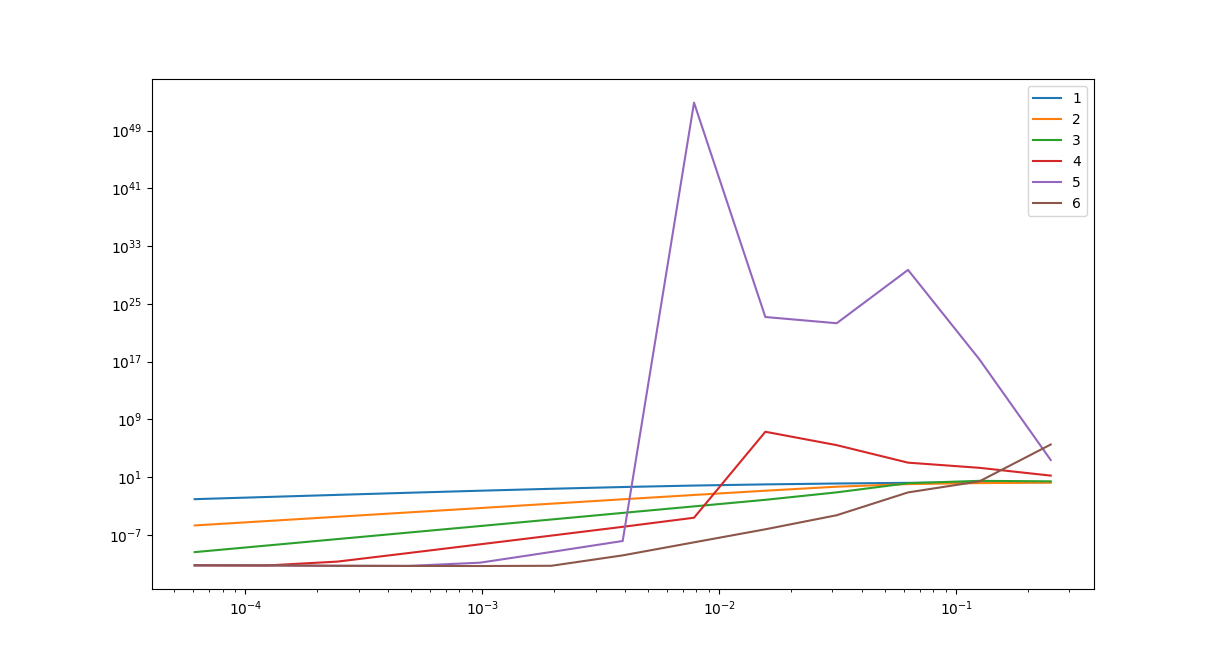
\includegraphics[width=0.5\textwidth]{bad_order_rates.png}
\end{figure}
Method 4 and 5 are presently the most underexlplored, and additional work will go into their assessment. 
Additionally, to assist in numerical stability, when high powers of the differentiation matrix are computed, the timestep is multiplied into each before exponentiation.

\section*{Finding convergence rates}
Suppose the error (for example, the inf-norm between the true solution and the approximate solution at the Chebyshev points) is $O((\triangle t)^k)$.
This means the error, defined to be $E := E(\triangle t)$ (we take the error to be a function of the time step size) is of the form
\begin{align*}
	E(\triangle t) = c (\triangle t)^{k}
\end{align*}
where $c$ is some constant.
We expect that when we halve $\triangle t$, $E(\frac{(\triangle t)}{2})$ will be reduced by $2^{k}$ i.e.
\begin{align*}
	E\Big( \frac{\triangle t}{2} \Big) = c \Big( \frac{\triangle t}{2} \Big)^{k}
\end{align*}
Dividing $E(\triangle t)$ by $E \Big( \frac{\triangle t}{2} \Big)$, we get
\begin{align*}
	\frac{ E (\triangle t) }{ E \Big( \frac{\triangle t}{2} \Big) } & = 2^{k}
\end{align*}
Taking $\log$ base $2$ of both sides, we get
\begin{align*}
	\log \Bigg( \frac{ E (\triangle t) }{ E \Big( \frac{\triangle t}{2} \Big) } \Bigg) & = k
\end{align*}
If we have a sequence of time step sizes $\triangle t_{1}, \triangle t_{2}, \hdots, \triangle t_{m}$ and their associated errors $E_{1}, E_{2}, \hdots, E_{m}$, we can recover what the order of convergence $k$ is by repeating the above calculations with $\triangle t_{1}$ and $E_{1}$, with $\triangle t_{2}$ and $E_{2}$, and so forth.
\par 
There is another way to compute the convergence rate.
We again assume that the error $E := E(\triangle t)$ is of the form
\begin{align*}
	E(\triangle t) & = c (\triangle t)^{k}
\end{align*}
Taking the natural log of both sides of the above expression, we get
\begin{align*}
	\log (E(\triangle t)) & = \log(c) + k \log(\triangle t)
\end{align*}
If we have multiple, distinct values of $\triangle t$ i.e. $\triangle t_{1}, \triangle t_{2}, \hdots, \triangle t_{m}$ and the associated errors $E_{1}, E_{2}, \hdots, E_{m}$, we can obtain a system of equations in $\log(c)$ and $k$ i.e.
\begin{align*}
	\begin{bmatrix}
		1 & \log(\triangle t_{1}) \\
		1 & \log(\triangle t_{2}) \\
		\vdots & \vdots \\
		1 & \log(\triangle t_{m})
	\end{bmatrix}
	\begin{bmatrix}
		\log(c) \\
		k
	\end{bmatrix}
	& = 
	\begin{bmatrix}
		\log(E_{1}) \\
		\log(E_{2}) \\
		\vdots \\
		\log(E_{m})
	\end{bmatrix}
\end{align*}
We denote the matrix on the left to be $\mat{A}$, the vector on the right to be $\vec{b}$, and the solution vector to be $\vec{x}$.
\par 
This is an over-determined linear system, so we will not be able to find an exact solution to $\mat{A} \, \vec{x} = \vec{b}$.
We can instead solve the normal equations.
If we multiply both sides $\mat{A} \, \vec{x} = \vec{b}$ by $\mat{A^{T}}$, we obtain the following system
\begin{align*}
	\mat{A^{T}} \, \mat{A} \, \vec{x} & = \mat{A^{T}} \, \vec{b}
\end{align*}
Since we assumed  $\triangle t_{1}, \triangle t_{2}, \hdots, \triangle t_{m}$ to be distinct, the columns of $A$ are linearly independent and $\mat{A^{T}} \, \mat{A}$ is non-singular.
Furthermore, $\mat{A^{T}} \, \mat{A}$ is a $2 \times 2$ matrix, which we can easily invert, and we are able to find the solution $\vec{x}$ in the least squares sense.

\section*{Testing the time-stepping code}
Suppose our PDE is of the form 
\begin{align*}
	\mathcal{L}(q) & = f
\end{align*}
It is often the case that we do not know the solution to such PDE's.
In order to test our code, we can use the \underline{method of manufactured solutions}.
We can come up with a dummy solution, $q^{*}$ and apply $\mathcal{L}$ to $q^{*}$ to obtain a different PDE i.e.
\begin{align*}
	\mathcal{L}(q^{*}) & = g
\end{align*}
Since we know $q^{*}$ exactly, we can test our code on the above PDE and compute the error between the approximate solution and true solution.
If it is the case that our code fails to find numerically accurate solutions even when we know the exact solution to the modified PDE, then we know our code will not find numerically accurate solutions to the original PDE. 
\par
This method is fairly robust for simple PDE's, but we have to be careful when our PDE gets more complicated. 
We also have to be mindful of initial conditions and boundary conditions when coming up with our manufactured solution.	

%June 6
$\quad$To start off today, we were working on the code from yesterday and trying to figure out what we were doing wrong. We started off trying different ways of zeroing out the last row and column of the matrix to see which method was working the best. We eventually figured out that we needed to zero out the last row and column of the matrix before we took the matrix to a power. When we figured this out, we figured out that our code was in fact working, but that the equation that we were using was unstable at the higher orders. Therefore, this equation was useless for what we were trying to accomplish and we were back to square one with finding an equation.

\section*{Stability analysis}
We analyze the model problem
\begin{align*}
	\hat{q}_{, t} & = \lambda \hat{q}(t)
\end{align*}
where $\lambda \in \mathbb{C}$ and $\text{Re}(\lambda) < 0$.
\par
We can write the solution at time $t$ using a reverse Taylor expansion i.e.
\begin{align*}
	q(t) & = \Big( 1 - \triangle t q_{, t}(t + \triangle t) + \frac{(\triangle t)^{2}}{2} q_{, t, t}(t + \triangle t) - \frac{(\triangle t)^{3}}{6} q_{, t, t, t}(t + \triangle t) + \hdots \Big) \\
		 & = \Big( 1 - \triangle t \lambda  + \frac{(\triangle t)^{2}}{2} \lambda^{2} - \frac{(\triangle t)^{3}}{6} \lambda^{3} + \hdots \Big) q(t + \triangle t) \\
		 & = \Big( 1 - z  + \frac{1}{2} z^{2} - \frac{1}{6} z^{3} + \hdots \Big) q(t + \triangle t)
\end{align*}
where we have defined $z := \triangle t \lambda$.
We can write the solution at the next time step (denoted $q^{n+1}$) as follows
\begin{align*}
	q^{n+1} & = \Bigg( \frac{1}{1 - z  + \frac{1}{2} z^{2} - \frac{1}{6} z^{3} + \hdots} \Bigg) \, q^{n}
\end{align*}
In order for $q^{n+1}$ to not blow up, we have to ensure that the magnitude of the factor $\Bigg( \frac{1}{1 - z  + \frac{1}{2} z^{2} - \frac{1}{6} z^{3} + \hdots} \Bigg)$ is less than or equal to $1$ i.e. we have to ensure that 
\begin{align*}
	\left\lvert \Bigg( \frac{1}{1 - z  + \frac{1}{2} z^{2} - \frac{1}{6} z^{3} + \hdots} \Bigg) \right\rvert  \leq 1 
\end{align*}
or equivalently,
\begin{align*}
	\left\lvert \Bigg( 1 - z  + \frac{1}{2} z^{2} - \frac{1}{6} z^{3} + \hdots \Bigg) \right\rvert \geq 1
\end{align*}
From earlier, we are working with the semi-discrete form of the advection equation
\begin{align*}
	\frac{\partial}{\partial t} \hat{q} & = \mat{D_{N}} \, \vec{\hat{Q}}
\end{align*} 
We had been using reverse Taylor expansions to compute approximate solution values at the $(n+1)^{th}$ time step i.e.
\begin{align*}
	\vec{\hat{Q}}^{n+1} & = \Bigg( \mat{I} + \triangle t \mat{D_{N}} 
										   + \frac{(\triangle t)^{2}}{2} \mat{D_{N}}^{2} 
										   + \frac{(\triangle t)^{3}}{6} \mat{D_{N}}^{3}
										   + \hdots \Bigg)^{-1} \vec{\hat{Q}}^{n}
\end{align*}
where we truncate the matrix before we invert it for computational purposes i.e. the first order implicit method corresponds to multiplication with $\Bigg( \mat{I} + \triangle t \mat{D_{N}} \Bigg)^{-1}$, the second order implicit method corresponds to multiplication with $\Bigg( \mat{I} + \triangle t \mat{D_{N}} + \frac{(\triangle t)^{2}}{2} \mat{D_{N}}^{2} \Bigg)^{-1}$, and so forth.
\par 
Within our code, we noticed first order, second order, and third order convergence rates with the corresponding methods, but the fourth, fifth, and sixth order implicit methods did not converge as expected. 
This is due to the fact that the fourth, fifth, and sixth order methods are not A-stable, as seen by looking at their stability plots.
\begin{figure}[H]
	\centering
	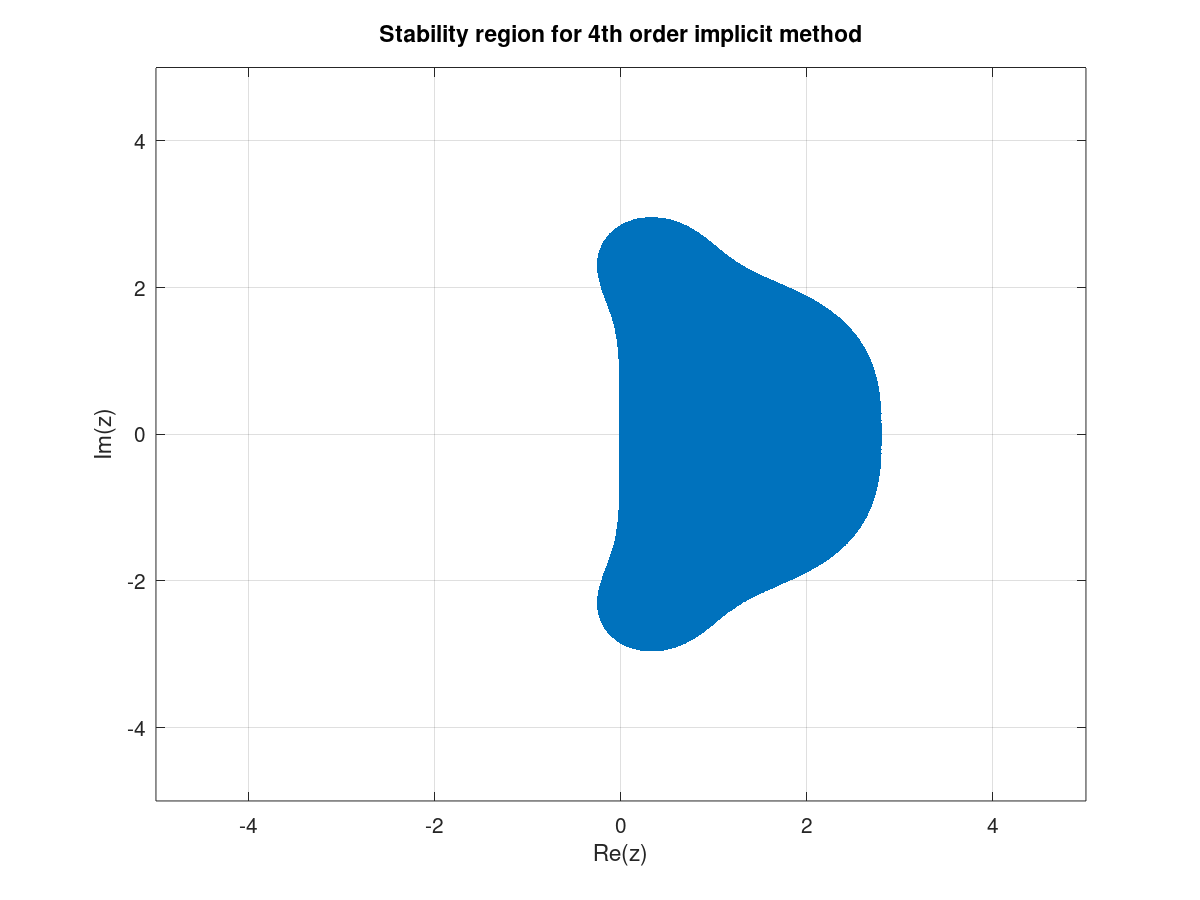
\includegraphics[width=0.75\textwidth]{fourth_order_stab_region.png}
\end{figure}

\begin{figure}[H]
	\centering
	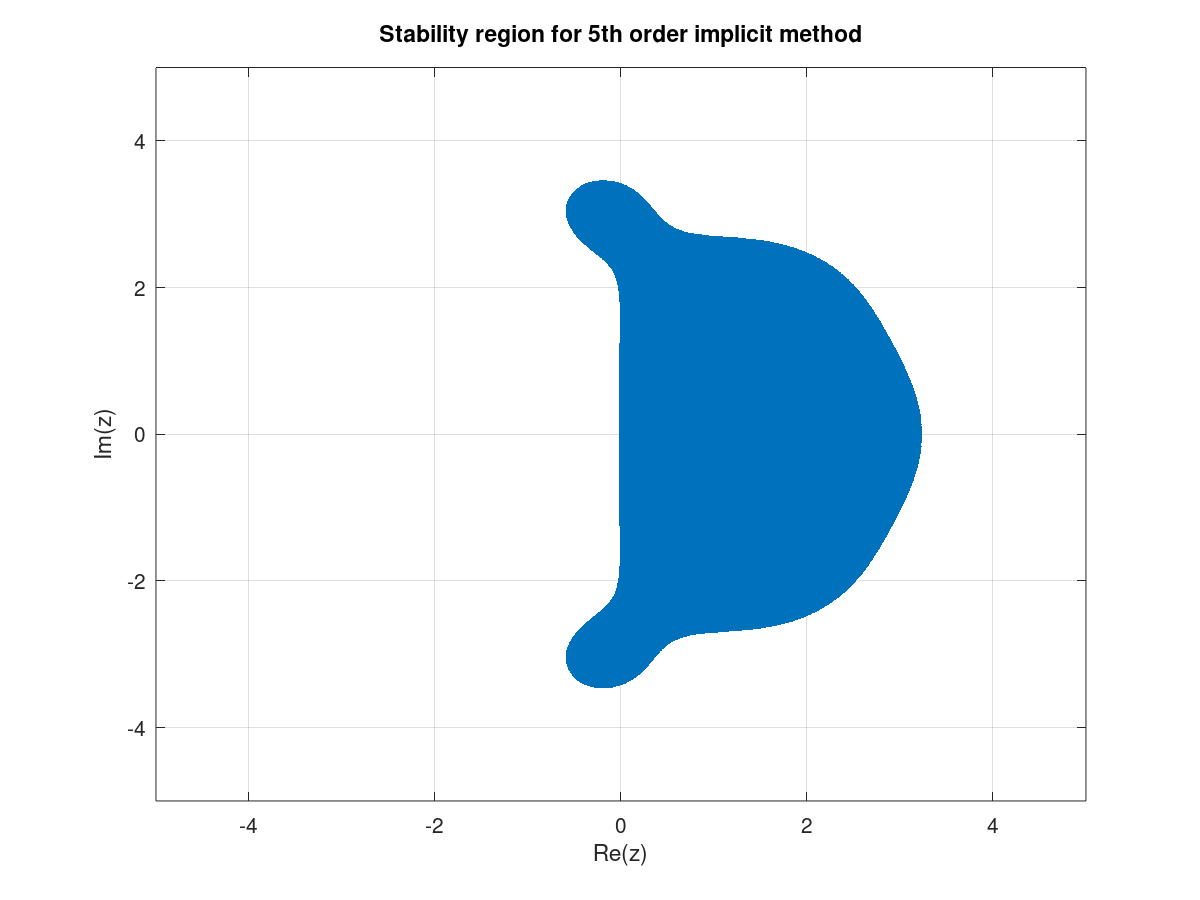
\includegraphics[width=0.75\textwidth]{fifth_order_stab_region.png}
\end{figure}

\begin{figure}[H]
	\centering
	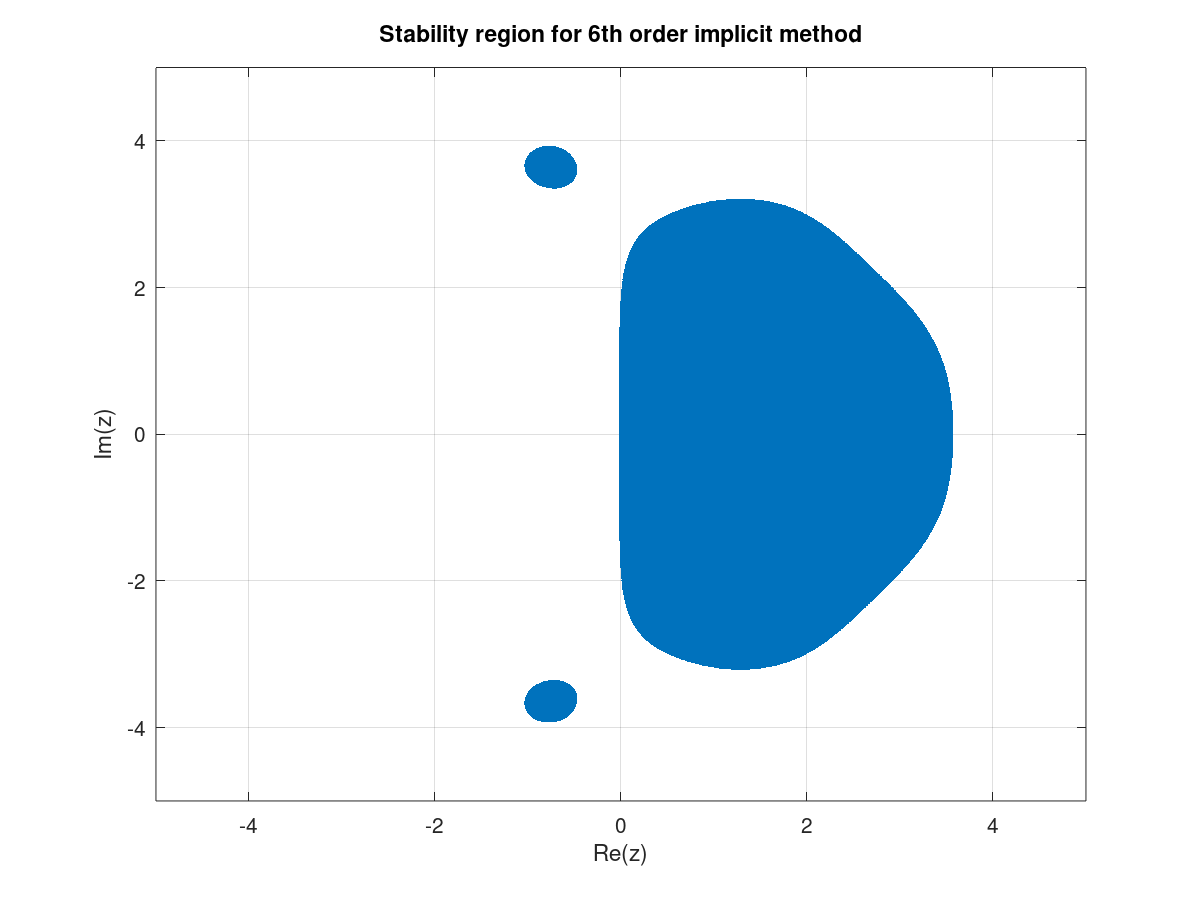
\includegraphics[width=0.75\textwidth]{sixth_order_stab_region.png}
\end{figure}
Because of this, we decided to use backward Euler method as our first order implicit method and the trapezoidal rule as our second order implicit method. 

\section*{New fourth-order time stepping method}
Later in the day, Dr. Rossmanith found a fourth order implicit method that is an extension of the trapezoidal rule. 
\par 
Suppose that our ODE is given by
\begin{align*}
	q_{, t}(t) & = f(t, q(t))
\end{align*}
with the appropriate initial conditions and boundary conditions.
The fourth-order scheme is given by
\begin{align*}
	q^{n+1} = q^{n} + \frac{\triangle t}{2} \Bigg( q_{, t}^{n} + q_{, t}^{n + 1} \Bigg)
					+ \frac{(\triangle t)^{2}}{12} \Bigg( q_{, t, t}^{n} - q_{, t, t}^{n + 1} \Bigg)
\end{align*}
The stability region of the trapezoidal rule is the entire left half of the complex plane.
The stability region of the above rule is also the entire left half of the complex plane.
\par 
We also discussed different time-stepping schemes.
If we assume our ODE is given by
\begin{align*}
	q_{, t}(t) & = f(q(t))
\end{align*}
the second order explicit Runge-Kutta method is given by 
\begin{align*}
	q^{*} & = q^{n} + \triangle t f(q^{n}) \\
	q^{n+1} & = q^{n} + \frac{\triangle t}{2} \Big( f(q^{*}) + f(q^{n}) \Big) 
\end{align*}
We also discussed the difference between \underline{diagonally implicit Runge-Kutta} (DIRK) and \underline{fully implicit} Runge-Kutta schemes.
Roughly speaking, a DIRK method is of the form
\begin{align*}
	q^{(1)} & = q^{n} + c_{1} \triangle t f(q^{n}, q^{(1)}) \\
	q^{(2)} & = q^{n} + c_{2} \triangle t f(q^{n}, q^{(1)}, q^{(2)}) \\
	q^{(3)} & = q^{n} + c_{3} \triangle t f(q^{n}, q^{(1)}, q^{(2)}, q^{(3)}) \\
	        & \vdots 
\end{align*}
We see each computation is ``implicit" (for example, in order to compute $q^{(1)}$, we need to know information about $q^{(1)}$), but each computation is independent of future computations.
On the other hand, a fully implicit Runge-Kutta method is of the form
\begin{align*}
	q^{(1)} & = q^{n} + c_{1} \triangle t f(q^{n}, q^{(1)}, q^{(2)}, q^{(3)}) \\
	q^{(2)} & = q^{n} + c_{2} \triangle t f(q^{n}, q^{(1)}, q^{(2)}, q^{(3)}) \\
	q^{(3)} & = q^{n} + c_{3} \triangle t f(q^{n}, q^{(1)}, q^{(2)}, q^{(3)}) \\
	        & \vdots
\end{align*}
We see that each update computation is potentially coupled with past and future computations.
Fully implicit Runge-Kutta methods tend to have better have convergence rates than DIRK methods, but these fully implicit methods are harder to implement compared to the DIRK methods due to how tightly coupled the updates are in the fully implicit methods. 

The next problem of interest is a coupled system of hyperbolic equations.
Specifically, we wrote code to solve the following system:
\begin{align*}
	\begin{bmatrix}
		q_1\\
		q_2
	\end{bmatrix}_{,t} + 
	\begin{bmatrix}
		0 & 1 \\
		1 & 0
	\end{bmatrix}
	\begin{bmatrix}
		q_1 \\
		q_2
	\end{bmatrix}_{,x} = 
	\begin{bmatrix}
		0 \\
		0
	\end{bmatrix}
\end{align*}
These equations are derived from the 1D wave equation, $\phi_{,t,t} - \phi_{,x,x} = 0$ using the substitutions $q_1 = -\phi_{,t}$ and $q_2 = \phi_{,x}$

The boundary conditions of this equation must be handled in the same way as the previously solved advection equation, being built in to the spatial discretization scheme.
As a result, the 2 equations must be decoupled prior to discretization in space, being done using their eigenvalue decomposition.

Taking the above matrix to be $\mat{A}$, using the derivation of 
\begin{align*}
	\mat{A} - \lambda \mat{I}) = 
	\begin{bmatrix}
		-\lambda & 1 \\
		1 & \lambda
	\end{bmatrix}
\end{align*}
it is found the eigenvalues of $\mat{A}$ are $\lambda = \pm 1$, with associated eigenvectors $[\quad 1]^T$ and $[-1\quad1]^T$ respectively.
As a result, the equations are decomposed into the following system
\begin{align*}
	\begin{bmatrix}
		q_1\\
		q_2
	\end{bmatrix}_{,t} + 
	\begin{bmatrix}
		1 & 1 \\
		-1 & 1
	\end{bmatrix}	
	\begin{bmatrix}
		-1 & 0 \\
		0 & 1
	\end{bmatrix}
	\begin{bmatrix}
		\frac{1}{2} & \frac{-1}{2} \\
		\frac{1}{2} & \frac{1}{2}
	\end{bmatrix}
	\begin{bmatrix}
		q_1 \\
		q_2
	\end{bmatrix}_{,x} = 
	\begin{bmatrix}
		0 \\
		0
	\end{bmatrix}
\end{align*}
and the appropriate transformation in coordinates being made:
\begin{align*}
	\begin{bmatrix}
		w_1\\
		w_2
	\end{bmatrix}_{,t} + 
	\begin{bmatrix}
		-1 & 0 \\
		0 & 1
	\end{bmatrix}
	\begin{bmatrix}
		w_1 \\
		w_2
	\end{bmatrix}_{,x} = 
	\begin{bmatrix}
		0 \\
		0
	\end{bmatrix}
\end{align*}
Under this scheme, the following are true:
\begin{align*}
	q_1 = w_1 + w_2 \quad &\quad \quad w_1 = \frac{1}{2}(q_1 - q_2)\\
	q_2 = w_2 - w_1 \quad &\quad \quad w_2 = \frac{1}{2}(q_1 + q_2)\\
\end{align*}
and the resulting decoupled advection equations can be solved with the same spectral differentiation matrix, provided the appropriate boundary conditions are enforced.
Due to the particular decomposition, the inflow for $w_1$ occurs on the left-hand side of the domain, and the inflow for $w_2$ occurs on the right.

$\quad$Then, we were working on coding with our new equations. We were trying to accomplish two things: test the stability of our new equations and solve the wave equation. When we were testing the stability of our new equations, we were working in the $\texttt{beuler\_advection.py}$ file. We have parts of the old equations commented out with the new equations in their places. With our new equations, we only have 3 orders of accuracy: first, second, and fourth. Since fourth order accuracy is still fairly accurate, we decided that we can move onto working with the wave equation instead of trying to figure out another equation to get up to sixth order accuracy. \\

$\quad$We decided that we needed a second file to work with the wave equation so that we still had our $\texttt{beuler\_advection.py}$ file. We named this file $\texttt{wave\_equation.py}$. We were mostly just editing out $\texttt{beuler\_advection.py}$ file, so a lot of our code is a repeat of code that we had previously. In $\texttt{wave\_equation.py}$, we defined a function called $\texttt{wave}$ that we are using to solve the wave equation. 

$$\texttt{q1, q1, s = wave( tf, N, dt, p0, pt0,  domain=[-1, 1], order=2, plot=True)}$$ 

There were some major changes with the code from the $\texttt{beuler\_advection.py}$ file, though. One major change is that now, instead of just having one equation to work with, we have two. In addition to the fact that we have two equations, they need to do different things. So, we needed two values for everything that we did in the $\texttt{beuler\_advection.py}$ file. \\
$\quad$We created two matrices, while still keeping the original the same, had two boundary conditions, had two lines of code in each order statement, and had two sets of transition equations to transition $w_1$ and $w_2$ to $q_1$ and $q_2$ and vice versa. We worked through writing all of the equations and at first, things were not working the way that we had hoped they would. But, after a simple switch of $w_1$ and $w_2$, things seemed to be working again. \\
$\quad$At this point in time, we decided that we should try and figure out how to get our solved $q_1$ and $q_2$ valued back into their original form, $\phi$. After staring at the problem for a while, we decided to try and see if adding $w_1$ and $w_2$ was the solution we were looking for. However, we looked further and figured out that $w_1 + w_2 = q_1$. Although our plotting of these values seemed to be doing something that we were looking for, we knew that it wasn't right. We eventually deduced that we were not going to be able to figure this out on our own, and asked Christine for help. The only thing that she could think to do was to interpolate our chebyshev values, so she reached out to a colleague, Jay, for assistance. Jay agreed with Christine and mentioned that there is a MATLab program that can do large-scale interpolation. However, since we are using Python, that wasn't helpful to us. We decided to sleep on it, while partially hoping that we do not need to convert the solved $q_1$ and $q_2$ back into $\phi$.

%June 7
\subsection{Application}

The application of interest to us is Radiative Transfer, a model for subatomic particles (specifically photons and neutrons) propogating in a homogenous medium.
The principle governing equation is as follows:
\begin{align*}
	F_{,t} + \vec{\Omega} \cdot \vec{\nabla}F + \sigma F = \frac{\sigma}{4\pi}\int_{\mathbb{S}^2}F\,d\vec\Omega
\end{align*}
We want to solve for the distribution of particles
\begin{align*}
	F( t, \vec{x}, \vec{\Omega}) : \quad \R^+ \times \R^3 \times \mathbb{S}^2 \to \R
\end{align*}
where $t$ is time, $\vec{x}$ is a position, and $\vec{\Omega}$ are angular variables.

In many ways, this equation is relatively simple, consisting of two "types" of terms.
The first of these is $ \vec{\Omega} \cdot \vec{\nabla}F $, which determines the advective character of the particles.
This is essentially transport with velocity $\vec{\Omega}$ (Note that $||\vec{\Omega}|| = 1$, thus all particles have speed exactly equal to 1).

The other terms can be combined into the collision term 
\begin{align*}
	\sigma\left(\frac{\sigma}{4\pi}\int_{\mathbb{S}^2}F\,d\vec\Omega - F\right).
\end{align*}
As an explanation for this terms effect on $F$, consider the following simple ordinary differential equation:
\begin{align*}
	F_{,t} = \sigma( G - F ).
\end{align*}
The solution to this equation is $F(t) = G + ce^{-\sigma t}$, which approaches $G$ as $t$ approaches infinity.
Analogously, this term in our model causes $F$ to "approach" $\frac{\sigma}{4\pi}\int_{\mathbb{S}^2}F\,d\vec\Omega\,$ as $t\to \infty$.
Moreover, because $\frac{\sigma}{4\pi}\int_{\mathbb{S}^2}F\,d\vec\Omega\,$ is equivalent to the angular average of the particles, this term indicates that the collisions in the system removes its angular dependence.
In other words, the particles are uniform across angles, and form an isotropic state.

When arranged into the following form, the model becomes a linear transport equation:
\begin{align*}
	F_{,t} + \vec{\Omega} \cdot \vec{\nabla}F = \sigma \left(\frac{\sigma}{4\pi}\int_{\mathbb{S}^2}F\,d\vec\Omega - F\right)
\end{align*}

However, while the PDE can be expressed simply, it is far from trivial. 
In particular, it is still a distribution functino in as many as $ 1 + 5$ dimensions.
This makes it fall under the influence of the curse of dimensionality, in which computational cost increases exponentially with dimension.
Typically, a problem that can be solved in $O(N)$ in 1D, must be solved in $O(N^d)$ in $d$-dimensions.
As a result some simplifications must be done on this problem to make it solvable in a resonable computation time.

$P_N$ approximation to radiative transfer:

Idea: expand angular part of the solution in terms of spherical harmonics.

\begin{figure}[H]
\centering
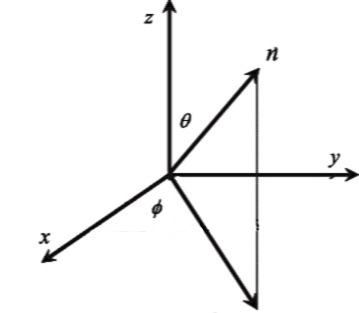
\includegraphics[width=0.8\textwidth]{spherical_harmonics_graph.jpg}
\caption{The image above shows the representation of where $\theta$ and $\phi$ are in relation to a graph.}
\end{figure}

$\theta$ is the co-latitutde and ranges from $0 \leq \theta \leq \pi$ where $0$ is the north pole and $\pi$ is the south pole. 

$\phi$ is the longitute and ranges from $0 \leq \phi \leq 2\pi$.

Let $\mu = \cos(\theta)$. Then $\mu \in [-1,1]$ where $-1$ corresponds to the south pole and $1$ corresponds to the north pole.

\begin{align*}
Y^m _l (\mu, \phi) = \sqrt{\frac{(2l+1)(l-m)!}{4\pi (l+m)!}} P^m _l (\mu) e^{im\phi} \\
\text{Where} P^m _l (\mu) \text{is the associated Legendre function.} \\
\text{Note: } Y^m _l = (-1)^m Y^{-m} _l \\
\end{align*}

\begin{align*}
\text{Let} F(t, \vec{x}, \vec{\Omega}) &= \sum^{\infty}_{l=0} \sum^{l}_{m=-l}  F^m _l (t, \vec{x}) Y^m _l (\mu, \phi) \\
F(t, \vec{x}, \vec{\Omega} &\approx \sum^{N}_{l=0} \sum^{l}_{m=-l} F^m _l (t, \vec{x}) Y^m _l (\mu, \phi)
\end {align*}

The plan is to use spherical harmonics because they are orthonormal on the unit sphere:
\begin{align*}
\int_{s^2} Y^m _l (\mu, \phi) Y^{m'} _{l'} (\mu, \phi) d\vec{\Omega} = \int_{m m'} \int_{l l'}
\end{align*}

Plug $F(t, \vec{x}, \vec{\Omega} \approx \sum^{N}_{l=0} \sum^{l}_{m=-l} F^m _l (t, \vec{x}) Y^m _l (\mu, \phi)$ into the radiative transfer equation, then multiply by $Y^{m'} _{l'}$ then integrate over the unit sphere. Then, after lots of algebra, you are left with linear hyperbolic equations. \\

Let 
\begin{align*}
\vec{F} := (F^0 _0, F^0 _1, F^0 _2, \dots , F^0 _N, F^1 _1, F^1 _2, F^1 _N, \dots , F^N _N)
\end{align*}

Note: These are all functions, $F^m _l (t, \vec{x})$.

Not all functions are in the list since there is some symmetry in the coefficients mentioned above. The unknown coefficients are as follows:

\begin{align*}
l = 0 \quad & F^0 _0 \\
l = 1 \quad & F^0 _1 \quad F^1 _1 \\
l = 2 \quad & F^0 _2 \quad F^1 _2 \quad F^2 _2 \\
l = 3 \quad & F^0 _3 \quad F^1 _3 \quad F^2 _3 \quad F^3 _3 \\
l = 4 \quad & F^0 _4 \quad F^1 _4 \quad F^2 _4 \quad F^3 _4 \quad F^4 _4
\end{align*}

The total number of unknowns is:
\begin{align*}
\sum^N _{l=0} \sum^l _{m=0} i = \frac{1}{2} (N^2 + 3N) + 1 = O(N^2)
\end{align*}

\section*{Daily update on code}
Today, we worked on generalizing the one-dimensional wave equation code so that it would solve more than two advection equations with absorbing boundary conditions simultaneously.
We begin with the potentially coupled system of equations we obtain by transforming the wave equation
\begin{align}
	\vec{q}_{, t} + \mat{A} \, \vec{q}_{, x} & = \vec{0}
\end{align}
We assume that $\mat{A}$ is a symmetric $M \times M$ matrix with real entries and that we can take the spectral decomposition of $\mat{A}$ as follows
\begin{align}
	\mat{A} & = \mat{R} \, \mat{\Lambda} \, \mat{R^{-1}}
\end{align}
where $\mat{R}$ is the matrix whose columns are the eigenvectors of $\mat{A}$ and $\mat{\Lambda}$ is the diagonal matrix whose diagonal entries contain the eigenvalues of $\mat{A}$.
We can then use the above decomposition to write the original system of equations as
\begin{align}
	\vec{q}_{, t} + \mat{R} \, \mat{\Lambda} \, \mat{R^{-1}} \, \vec{q}_{, x} & = \vec{0}
\end{align}
We multiply the above equation through by $\mat{R^{-1}}$ to obtain
\begin{align}
	\mat{R^{-1}} \, \vec{q}_{, t} + \mat{\Lambda} \, \mat{R^{-1}} \, \vec{q}_{, x} & = \vec{0}
\end{align}
Since $\mat{R}$ (and $\mat{R^{-1}}$) are constant matrices, differentiation with respect to time or space will not affect these matrices, so can make the following substitution
\begin{align}
	\vec{w} & = \mat{R^{-1}} \, \vec{q}
\end{align}
We can now rewrite the equation as
\begin{align} 
	\vec{w}_{, t} + \mat{\Lambda} \, \vec{w}_{, x} & = \vec{0}
\end{align}
The $i^{th}$ equation in the above system reads as 
\begin{align}
	w_{i, t} + \lambda_{i} w_{i, x} & = 0
\end{align}
We can obtain the semi-discrete form of the above equation by replacing the partial derivative with respect to space with $\mat{D_{N}}$ (where $N + 1$ is the number of Chebyshev points we use) and discretizing the solution $w_{i}$
\begin{align}
	\vec{w_{i}}_{, t} + \lambda_{i} \mat{D_{N}} \, \vec{w_{i}} & = 0
\end{align}
Depending on the sign of $\lambda_{i}$, we need to modify $\mat{D_{N}}$ to include the absorbing boundary conditions i.e. if $\lambda_{i}$ is negative, we need to zero out the first column and row of $\mat{D_{N}}$ and vice versa. 
At this point, we can discretize the above equation with respect to time and apply backward Euler, the trapezoidal rule, or the fourth order extension of the trapezoidal rule to time-step.

%June 10
We began by setting up the matrix coefficients that represent the system of equations described by (8) and (9) in the Brunner, Holloway paper, reproduced below.

The following represents the three-dimensional Boltzmann equation, for $0 \leq l < \infty$ and $-l \leq m \leq l$.
and for $m \neq 0$:
\begin{align*}
	\frac{\partial}{\partial t}\psi_{l}^{m} &+ \frac{1}{2}\frac{\partial}{\partial x}
	(
	-C_{l-1}^{m-1}\psi_{l-1}^{m-1} + 
	D_{l+1}^{m-1}\psi_{l+1}^{m-1} + 
	E_{l-1}^{m+1}\psi_{l-1}^{m+1} + 
	-F_{l+1}^{m+1}\psi_{l+1}^{m+1} 
	)\\ &+ 
	\frac{\partial}{\partial z}
	(
	A_{l-1}^{m}\psi_{l-1}^{m} + 
	B_{l+1}^{m}\psi_{l+1}^{m}
	) + \Sigma_t\psi^{m}_{l} = 0.
\end{align*}

For $m = 0$:
\begin{align*}
	\frac{\partial}{\partial t}\psi_{l}^0 + 
	\frac{\partial}{\partial x}
	(
	E_{l-1}^{1}\psi_{l-1}^{1} + 
	-F_{l+1}^{1}\psi_{l+1}^{1} 
	) +  
	\frac{\partial}{\partial z}
	(
	A_{l-1}^{0}\psi_{l-1}^{0} + 
	B_{l+1}^{0}\psi_{l+1}^{0}
	) + \Sigma_t\psi^0_{l} = \Sigma_s\psi^0_0\delta_{l0}
\end{align*}

(The specific values for the coefficients $A_l^m$, $B_l^m$, etc. can be found in the paper by Brunner and Holloway)

Additionally, the identity $\bar{\psi_l^m} = (-1)^m\psi_l^{-m}$ takes advantage of each $\psi$ being real to remove terms with negative $m$.
Thus $m$ goes from $0$ to $l$ instead of $-l$ to $l$.
Under the $P_N$ approximation, it is assumed that $\psi_l^m = 0$ whenever $l > m$, $l < 0$, or $l > m$.
This results in the system of equations represented by the matrices produced by $\texttt{pn\_approx.py}$, which produces the matrices $A, B$, and $C$ in the following system:
\begin{align*}
	\vec{q}_{,t} + \mat{A}\,\vec{q}_{,x} + \mat{B}\,\vec{q}_{,z} = \mat{C}\,\vec{q}
\end{align*}
Unlike the paper by Brunner and Holloway, the functions $\psi_l^m$ are grouped by $l$ rather than $m$.
As a result, the following mapping from $(m, l)$ to equation number $p$ is used:
\begin{align*}
	p = \frac{l(l+1)}{2} + 1 + m
\end{align*}
This mapping causes the exact matrices produced in the paper by Brunner and Holloway and our own to be distinct, but only as permutations of one another.

In our code, named $\texttt{pn\_approx.py}$, we set functions for A, B, C, D, E, F that can be found in the Brunner Holloway paper on two-dimensional time dependent Riemann solvers for neutron transport in equations (4), (5), and (6). Then, we defined a python function, $\texttt{pn\_matrices}$, to loop through different values of $\ell$ and $m$ to create our matrices. In order for this to work correctly, we needed to have if statements for each type of value. This could be improved upon at a later time, but for now, it allows our code to run without causing issues with our $\ell$ and $m$ values to be less than $0$ or greater than $N$. We also imported the sys library of python in order to run different $N$ values from our terminal instead of having to change our code each time we tested a different $N$ value. \\

Note: $N$ is always a positive, odd integer. \\

We needed to only deal with one variable at a time instead of dealing with $m$ and $\ell$ at the same time. The following equation outlines a way that we were able to do that:

\begin{align*}
p = &\frac{\ell(\ell + 1)}{2} + 1 + m \\
\ell = &0, 1, 2, \dots, N \\
m = &0, 1, 2, \dots, \ell \\
1\leq p \leq &\frac{N(N + 1)}{2} + 1 + N \\
1\leq p \leq &\frac{N^2}{2} + \frac{3N}{2} +1
\end{align*}

The following are the two cases for our equations:

\begin{align*}
\text{For } m \neq 0 \text{:} \\
\psi_{p,t} + \frac{1}{2} \frac{\partial}{\partial x} [-C_{\ell - 1}^{m-1} \psi_{p-\ell-1} + D_{\ell + 1}^{m-1} \psi_{p + \ell} + E_{\ell - 1}^{m + 1} \psi_{p- \ell +1} - F_{\ell + 1}^{m+1} \psi_{p + \ell + 2} ] \\ + \frac{\partial}{\partial z} [A_{\ell - 1}^{m} \psi_{p-\ell} + B_{\ell + 1}^{m} \psi_{p+\ell+1}] + \sum_t \psi_p = 0 \\ \\
\text{For } m = 0 \text{:} \\
\psi_p + \frac{\partial}{\partial x}[E_{\ell - 1}^1 \psi_{p-\ell +1} + F_{\ell + 1}^1 \psi_{p+\ell+2}] + \frac{\partial}{\partial z}[A_{\ell - 1}^0 \psi_{p-\ell} + B_{\ell+1}^0 \psi_{p+\ell+1}] + \sum_t \psi_p = \sum_s \psi_1 \delta_{\ell 0}
\end{align*}

The goal is to have the average approach the $\psi_0^0$ value. When our $p = 1$, our average value is $\psi_0^0$. 

\begin{align*}
\psi_{p,t} = -\sum_t \psi_p \\
\psi_{1,t} = -\sum_t \psi_1 + \sum_s \psi_1
\end{align*}

Going forward, we need to make a $\widetilde{\mat{A}} (\omega) = \cos(\omega) \mat{A_x} + \sin(\omega) \mat{A_z}$. We then send $\widetilde{\mat{A}}$ to the code that we have to solve matrices of this form and repeat for multiple values of $\omega$. Then, we need to address the fact that we don't have a uniform mesh because we are using Chebyshev points, so methods like the discrete Radon transform (DRT) won't work the same. \\
The easier part of the Radon transform will be doing the forward Radon transform, since it is just integration. However, the inverse Radon transform will be where we will struggle. 

%June 11
Today, we settled on taking the physical domain for the radiative transfer problem to be the unit disk centered at $(0, 0)$ discretized by equispaced angles $\{ \omega_j \}_{j=1}^{N}$.
We discretize the line that makes an angle of $\omega_{j}$ with the positive x-axis for $j = 1, 2, \hdots, N$ using the Chebyshev points.
This results in the following picture
% \includegraphics[\width=0.5\textwidth]{imagefile}
Our transformed space should roughly look like the following
% \includegraphics[\width=0.5\textwidth]{imagefile}
\par 
To compute the Radon transform at angle $\omega_{j}$ at a point $s_{i}$ along the line defined by $\omega_{j}$, we compute the following line integral
\begin{align*}
	\hat{f}(s_{i}, \omega{j}) & = \int_{-\infty}^{\infty} f(s_{i} \cos (\omega_{j}) - z \sin (\omega_{j}), \, s_{i} \sin (\omega_{j}) + z \cos (\omega_{j})) \, dz
\end{align*}
in the $z$-direction.
Graphically, this is the line integral along the chord passing through $s_{i}$ and perpendicular to the line defined by $\omega_{i}$.
We first assume the function $f$ is compactly supported (here, we take this to mean that $f$ is zero outside of the unit disk).
To compute the above line integral, we have to first compute the $z$-coordinates of the endpoints of the aforementioned chord.
Note that the distance from the left endpoint of the chord to $s_{i}$ (denoted $r_{1}$) and the distance from the right endpoint of the chord to $s_{i}$ (denoted $r_{2}$) are equal i.e. $r_{1} = r_{2} = r$.
\par 
To compute $r$, we simply use the Pythagorean theorem.
Without loss of generality, we form a right triangle whose sides consist of the line from the origin to the left endpoint of the chord, the line from the origin to $s_{i}$, and the line from $s_{i}$ to the left endpoint of the chord.
We know that the distance from the origin to the left endpoint of the chord is $1$ because we are on the unit disk. 
Hence, $r = \sqrt{1 - s_{i}^{2}}$. 
\par 
Now, the above line integral becomes
\begin{align*}
	\hat{f}(s_{i}, \omega_{j}) & = \int_{-\infty}^{\infty} f(s_{i} \cos (\omega_{j}) - z \sin (\omega_{j}), \, s_{i} \sin (\omega_{j}) + z \cos (\omega_{j})) \, dz \\
	& = \int_{-r}^{r} f(s_{i} \cos (\omega_{j}) - z \sin (\omega_{j}), \, s_{i} \sin (\omega_{j}) + z \cos (\omega_{j})) \, dz
\end{align*}
In practice, we will not know how to compute the above line integral analytically, so we turn to approximating the integral using quadrature rules.
\par 
We can use Clenshaw-Curtis quadrature quadrature to approximate the definite integral of a continuous functions $f$ on the interval $[-1, 1]$ i.e.
\begin{align*}
	\int_{-1}^{1} f(x) \, dx & \approx \sum_{i=0}^{N-1} w_{i} f(x_{i})
\end{align*}
where $w_{i}$ is the $i^{th}$ quadrature weight and $x_{i}$ is the $i^{th}$ Chebyshev point ($i = 0, 1, \hdots, N-1$).
However, this rule (and most other quadrature rules) only approximate definite integrals from $[-1, 1]$, and we want to approximate definite integrals on an arbitrary interval $[a, b]$.
\par 
Let $\vec{t} = [ x_0 \quad x_1 \quad \hdots \quad x_N]^{T}$ be $(N+1)$ Chebyshev points on $[-1, 1]$.
We can rescale the entries of $\vec{t}$ to lie on $[a, b]$ as follows
\begin{align*}
	z(t) & = \frac{b+a}{2} + \frac{b-a}{2} \, t
\end{align*}
If we want to compute the definite integral of a continuous function $f$ on $[a, b]$, we can use the above substitution i.e.
\begin{align*}
	\int_{a}^{b} f(z) \, dz & = \frac{b-a}{2} \, \int_{-1}^{1} g(t) \, dt
\end{align*}
where $dz = \frac{b-a}{2} \, dt$ and $g : [-1, 1] \rightarrow [a, b]$ is defined as follows
\begin{align*}
	g(t) & = f \Bigg( \frac{b+a}{2} + \frac{b-a}{2} \, t \Bigg)
\end{align*}
\par 
We can approximate the line integral
\begin{align*}
	\int_{-r}^{r} f(s_{i} \cos (\omega_{j}) - z \sin (\omega_{j}), \, s_{i} \sin (\omega_{j}) + z \cos (\omega_{j})) \, dz
\end{align*}
by using the Clenshaw-Curtis quadrature rule in the $z$-direction and by using the substitution
\begin{align*}
	z & = \frac{r + (-r)}{2} + \frac{r - (-r)}{2} \\
	  & = rt \\
	dz & = r \, dt
\end{align*}
Thus,
\begin{align*}
	\int_{-r}^{r} f(s_{i} \cos (\omega_{j}) - z \sin (\omega_{j}), \, s_{i} \sin (\omega_{j}) + z \cos (\omega_{j})) \, dz & = 
	r \int_{-1}^{1} f(s_{i} \cos (\omega_{j}) - rt \sin (\omega_{j}), \, s_{i} \sin (\omega_{j}) + rt \cos (\omega_{j})) \, dt \\
	& \approx r \sum_{k=0}^{N} w_{k} f(s_{i} \cos (\omega_{j}) - rt_{k} \sin (\omega_{j}), \, s_{i} \sin (\omega_{j}) + rt_{k} \cos (\omega_{j}))
\end{align*}
Doing this for every angle $\omega_{j}$ and for every discretization point $s_{i}$ along the line defined by $\omega_{j}$, we can effectively approximate the Radon transform of the function $f$ defined on the unit disk centered at $(0, 0)$. 

We created a new Python file called $\texttt{radon\_transform\_v1.py}$. In this file, we coded definitions including $\texttt{clen\_curt(N)}$ and $\texttt{cc\_quad(f, a, b, N)}$. \\

In $\texttt{clen\_curt(N)}$ we coded the Clenshaw-Curtis Quadrature that is described in MATLAB code on page 128 of Trefethen's book. We did most of the code the exact same, but with Python style rather than MATLAB. We were required to decrease the value of $N$ by $1$ since Python starts counting at $0$ while MATLAB starts counting at $1$. The method that is used in Trefethan's book uses something similar to the Fast Fourier Transform. The $\texttt{clen\_curt(N)}$ function is used in determining the chebyshev points and the weights, which we bring into the $\texttt{radon}$ function that is described below. \\

In $\texttt{cc\_quad(f, a, b, N)}$ we coded a way to run a convergence test on the Clenshaw-Cutrist Quadrature so that we could test to see how well our code was doing the Clenshaw-Curtis Quadrature. Otherwise, we do not use $\texttt{cc\_quad(f, a, b, N)}$ to do anything else in our code at this point in time. 

Today we completed the code $\texttt{radon\_transform\_v1.py}$, a module that contains functions to compute numerical quadrature and the forwards radon transformation.
The functions $\texttt{clen\_curt}$ and $\texttt{cc\_quad}$ create the nodes/weights for the Clenshaw-Curtis quadrature and approximate the integral respectively.
Their function declarations and return types are as follows:
$$\texttt{x, v = clen\_curt(N)}$$
where $x$ are the nodes, $v$ are the weights, and $N$ is the number of points used in the approximation.
$$\texttt{approx = cc\_quad(f, a, b, N)}$$
where $f$ is the function to be integrated along $[a, b]$ using $N$ quadrature points.
$\texttt{clen\_curt}$ is copied nearly line for line from page 128 in the Trefethen text, translated from MATLAB.
The most notable difference is that Trefethen's version of the function computes the integral along $N$ intervals, rather than $N$ quadrature points.


The function $\texttt{radon}$ computes the forwards radon transformation.
Its declaration and return values are as follows:
$$\texttt{f\_hat = radon( f, Ns, Nw )}$$
where $f$ is the function to be approximated, $\texttt{Ns}$ and $\texttt{Nw}$ are the discretization level for $s$ and $\omega$ respectively, $\texttt{t\_hat}$ is the radon transformation at each of the above points, returned in an $\texttt{Ns}\times\texttt{Nw}$ array.
The discretization follows the method described above, in which each point is located on the unit circle, and the diameter determined by each $\omega$ is spanned by chebyshev points. 

Although the true radon transform computes an integral across the real values, the code assumes that the function to be approximated is zero outside of the unit circle.
As a result, the quadrature points are only placed along the appropriate chord.
Additionally, the length of this chord is calculated in order to appropriately scale the integration to match the weights given by $\texttt{clen\_curt}$, which are valid only from $[-1, 1]$. 
Finally, the discretization for $s$ and $\omega$ are returned in a meshgrid.
While this is comparatively inefficient, this allows for simple plotting of the space and transformation.

In the future, extra care should be taken to remove the nested for loop structure to improve the runtime of the code.
That being said, this calculation is only done once over the course of a single problem, being done more or less offline.

Moreover, this code makes the assumption that the function to be transformed, $f$, can be evaluated at arbitrary points. In practice, $f$ is only known at the specific discretization points described above.
As a result, the code must eventually be rewritten to accomodate this.
The current plan is to attempt this process using a higher order interpolation scheme on the points, then computing the radon transformation of the interpolant instead.
This way, an inverse radon transformation can more easily be created and applied.

%June 12
Today we attempted to complete the code in the module $\texttt{radon\_transform\_v2.py}$.
Similar to version 1, this module contains a functino $\texttt{clen\_curt}$ that returns the appropriate nodes and weights for Clenshaw-Curtis approximation, the source for which is identical.

The module also incldes a $\texttt{radon}$ function which has an identical declaration and return type as the 1st version, but has a different definition.
This function uses interpolation to evaluate the function to be transformed at only the discretization points provided.
As of yet, the code uses bilinear interpolation, but does so in the $s \times \omega$ plane as opposed to the typical $x \times y$ plane, where the discretization points are placed in a grid, albeit a non-uniform one.
Each point required for the quadrature in the radon transformation is approximated by its four nearest neighbors in this $d \times \omega$ plane.
Locating these four points is done using the $\texttt{numpy}$ function $\texttt{digitize}$, which categorizes values into the appropriate interval.
TO remove any issues of points located on the boundary, each point is peturbed inwardly to ensure each is located in the interior of such a rectangle.

Currently, this code returns artifacts when tested on a gaussian function. 
It is suspected that this can be avoided if the number of chebyshev points used in quadrature is less than the number of chebyshev points used for the discretization, but this is currently under investigation.

%June 13	
We knew from yesterday that our code, in file $\texttt{radon\_transform\_v2.py}$ was having some errors. We were able to reduce the errors by increasing the number of s points in our grid. However we still weren't getting our error to reduce as much as we would like. \\ \\
 Before we could try different methods to change our error, we had to make sure that we were finding a correct solution, so we compared our solution to the exact solution and to the solution that we had in $\texttt{radon\_transform\_v1.py}$ We were able to determine that the solution found in $\texttt{radon\_transform\_v1.py}$ was correct with minimal error. \\ \\
 Then, we ended up trying to change the area on which we were doing the bilinear interpolation, however we were still unable to get our error to an acceptable amount. At this point, we were also trying to see if a radiative basis function with $\phi = 1$ would work better. It seemed to have less error, but the error started to increase with more s points. We are unsure if the radiative basis function will work out for us in the long run with this odd error behaviour.

\section*{Radon transform of scaled Gaussians}
Today, Dr. Rossmanith showed us how to compute the Radon transform of a scaled Gaussian.
We know from Dean's textbook that the Radon transform of $f(x, y) = \exp (-(x^{2} + y^{2}))$ is given as follows
\begin{align*}
\hat{f} (s, \omega) & = \int_{-\infty}^{\infty} f(s \cos (\omega) - z \sin (\omega), s \sin (\omega) + z \cos (\omega)) \, dz \\
& = \sqrt{\pi} \exp(-s^{2})
\end{align*}
If we were trying to compute the Radon transform of a scaled Gaussian i.e. the Radon transform of $g(x, y) = \exp (\alpha (x^{2} + y^{2}))$, where $\alpha$ is a positive constant, we can do the following
\begin{align*}
\hat{g} (s, \omega) & = 
\end{align*}

As a part of our efforts to find a suitable alternative to the evidently buggy bilinear interpolation, other interpolation schemes were investigated.
Among them was Shepard's method, which in general constructs a global interpolant according to an inverse dsitance weighting.
In our case, each point at which the function needed to be evaluated was placed inside a grid-cell in $s \times \omega$ space, just as in the bilinear case.
Then, the interpolant is constructed based on the function values at those four points only. 
With limited testing, this method appeared to work about as well as the radial basis function attempted the previous day, but at a much cheaper computational cost.
That being said, the method had similar artifacts as well, and was quickly abandonded in place of the angular interpolation method tried next.

%June 14
The new plan is to have the point that we are looking at, and then calculate two points that straddle that point that are on omega values that we have our quadrature points on. We then find the s-value of those points. Then, we do 1-dimensional interpolations along the quadrature lines to find the value of the straddle points. At this point, we do angular interpolation to find what our actual point is. 

\begin{figure}[H]
\centering
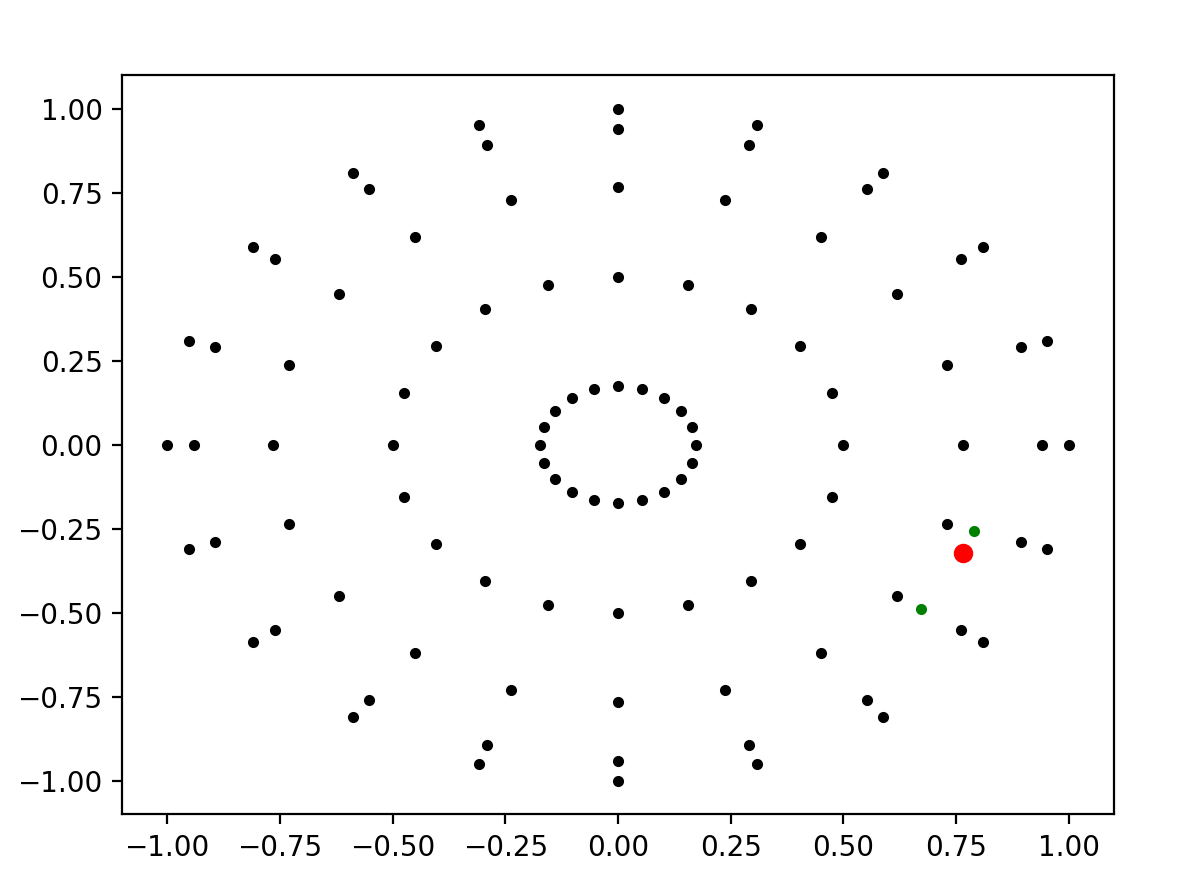
\includegraphics[width=0.8\textwidth]{StraddlePoints.jpg}
\caption{We want to find the red point. The green points are our straddle points. We need to find code to find the green points.}
\end{figure}

This should be a better method for accuracy since we are not looking for 4 points. \\

In order to code this, we need a 1-dimensional interpolation scheme. We want the interpolation scheme to be fast to evaluate and stable. 

\begin{align*}
P_n(x) = \frac{{\sum_{j = 0}^{n}}' \frac{(-1)^j f_j}{x-x_j}}{{\sum_{j = 0}^{n}}' \frac{(-1)^j}{x-x_j}} \\
{\sum _{j = 0}^{n}}' = \frac{1}{2}(j = 0) + (j = 1) + \dots + \frac{1}{2}(j = n)
\end{align*}

In the above equations, the x is equivalent to the s-value and the f is equivalent to the corresponding function value. A way to easier code the summation would be to rewrite it with normal summations.

\begin{align*}
P_n(x) = \frac{\sum_{j = 0}^{n} \alpha_j \frac{f_j}{x-x_j}}{\sum_{j = 0}^{n} \alpha_j\frac{1}{x-x_j}} \\
\alpha_0 = \frac{1}{2},\quad \alpha_{1:n-1} = (-1)^{1:n-1},\quad \alpha_n = \frac{1}{2} (-1)^n
\end{align*}

\section*{Implementation of new interpolation scheme}
We were not able to successfully compute the approximate Radon transform via bi-linear interpolation or Shepard's method.
Dr. Rossmanith showed us an alternative interpolation method.
\par 
We discretize the unit disk by discretizing the interval $[0, \pi]$ into $N_{\omega}$ many points, with a spacing of $\delta \omega$ between each point.
Along each angle $\omega_{i}$, we draw a line that goes through the origin of disk, and we discretize that line using $N_{s}$ many Chebyshev points.
For $N_{\omega} = 50$ and $N_{s} = 50$, the grid looks like the following
\begin{figure}[H]
	\centering
	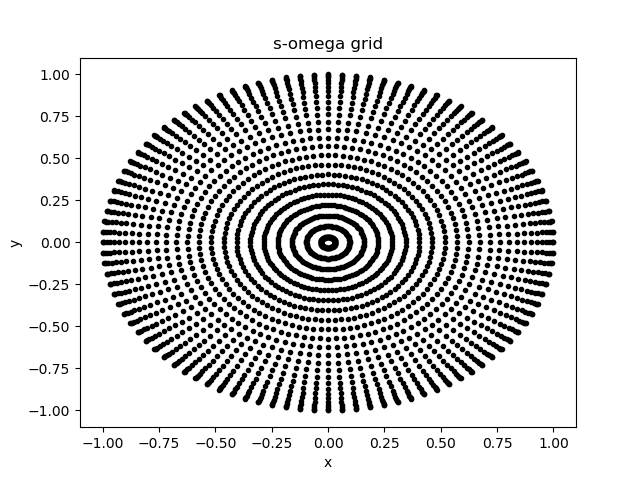
\includegraphics[width=0.75\textwidth]{s_omega_grid.png}
\end{figure}
We programmed the new interpolation scheme in \verb|radon_transfom_v5.py| within the function \verb|radon(f_vec, Ns, Nw, Nq)|, where the argument \verb|f_vec| is a $N_{\omega} \times N_s$ by $1$ long vector, \verb|Ns| is equal to $N_{s}$ i.e. the number of discretization points in the $s$-direction, \verb|Nw| is equal to $N_{\omega}$ i.e. the number of angles in the angular discretization, and \verb|Nq| is equal to the number of quadrature points we use to approximate the line integral at every mesh point.
\par
We originally define \verb|f_vec| to be a $N_{\omega} \times N_{s}$ matrix whose entries are $f$ (the function whose Radon transform we are taking) evaluated at all the points in $s$-$\omega$ discretization. 
We then flatten \verb|f_vec| to be a vector with $N_{\omega} \times N_{s}$ entries.
To convert between the position of a doubly indexed point in the mesh (for example, the point given by $(s_{j}, \omega_{i})$), we use the following linear index
\begin{align*}
	p & = i \times N_{s} + j
\end{align*}
The reason why we write \verb|f_vec| in this manner is because we eventually want to write the Radon transform of \verb|f_vec| as a matrix-vector multiplication.
\par
We obtain \verb|Ns| Chebyshev points and \verb|Nw| equispaced angles on the interval $[0, \pi]$, and we also compute \verb|Nq| many 

%June 17	
We make a new file $\texttt{radon\_transform\_v6.py}$ to take the nearest 4 points and interpolate between them to find our point. We copied $\texttt{radon\_transform\_v5.py}$ and then pasted it into $\texttt{radon\_transform\_v6.py}$ to have a base for our code. \\
When we were changing the code, we found our $\omega$ values by subtracting one from the previous $\omega$ lower index and adding one to the previous $\omega$ upper index. Then we did the same thing with our s-values and our function values. Then we had to code our interpolation method. We still had to code the summation from Friday into our interpolation method, so we created variables to do that, called $\texttt{p1, p2, p3, p4}$. We also had to create the angle $\theta_1$, which is the angle halfway between points $p_2$ and $p_3$. We accomplished this by taking the change in $\omega$ and dividing that by 2, then adding our $\omega_2$ to that. Then we plugged all of that information into our interpolation equation.

\section*{Fourth order interpolation scheme to compute Radon transform}
Dr. Rossmanith provided us with another interpolation scheme that is based off the earlier second order interpolation scheme from last week.
In this scheme, we make use of four points to compute the function value at a quadrature point.

In order to make the forward Radon transform more computationally efficient, effort was put into vectorizing the 2 point interpolation code in $\texttt{radon\_transform\_v5.py}$ into $\texttt{radon\_transform\_v5\_vec.py}$.
The motivation behind this vectorization was to group together all of the quadrature points used to calculate the Radon transform for a single discretization point.
This was mostly successful, although some calculations still had to be done within a for-loop.
Despite this, the changes made to the code made it run approximately four times as fast, and indicates that similar efforts should be put into vectorizing the other versions of the forward Radon transform.

%June 18	
Today we implemented the bi-conjugate gradient stabilized method, known as BiCGSTAB. We coded it in the file $\texttt{radon\_transform\_v6.py}$ in a function titled $\texttt{radon\_inverse}$. The psudeocode for our code came from page 91 of Iterative Methods for Solving Linear Systems by Anne Greenbaum. We then implemented the code in a tester file and observed how fast different functions converged. The more radially symmetric the function was, the faster the convergence rate. \\
We were able to observe a function that would not converge at a relatively quick rate. At that point, we determined that we needed to add a pre-conditioner. The question was, which pre-conditioner will work for our methods? At the end of the day, we had only found one that was quick to implement and made our functions converge at a quicker rate. This pre-conditioner, was to reduce the number of quadrature points for the inverse radon transform, as reducing the number of quadrature points for the forward radon transform makes an inaccurate radon transform. 

%June 19/20	
A significant portion of these days were spent making the Radon Transform software more efficient and fast.
This was primarily performed through Numpy vectorization.
Initially, the quadrature used to calculate the Radon Transform for a particular discretization point was vectorized, referred to as "vectorized in $q$".
This resulted in approximately a 10x speedup.
Next, the code was fully vectorized, being vectorized in $s$, $\omega$, and $q$.
For trivially coarse domains, this made the code significantly faster. 
However, for any reasonably sized domain, this vectorization caused the overall calculation to take either more time, or not compute at all due to memory constraints.
The unexpected slow-down in runtime is likely the result of cache issues, but the exact causes were not investigated fully.
To alleviate these issues, we attempted to vectorize the code only in $\omega$ and $q$, having the effect of computing the radon transform for entire diameters of the domain at once.
While this did not have the same memory issues as the original method, it remained only mildly more efficient at best, and slower at worst.
As a result, the version of the software vectorized in $q$ has become the de-facto radon transform to be used in future work.

When we were trying to create our pre-conditioner matrix using a radially symmetric function so that we wouldn't have $\omega$ dependence, we ran into singular matrix issues. When we printed out the matrix to try to figure out why, we noticed that the four quadrants of the matrix were mirrors of each other. \\
Our attempt to fix this was to cut out the upper right and the lower left quadrants to make all of the rows of the matrix unique. This was tricky to code, as we were looping through all Ns points, but we needed the second half of Ns points to look at the first half to find their values. Once we had this coded, we tested it as a pre-conditioner, and it made our condition number slightly better, but ultimately this matrix was not the pre-conditioner that we were hoping for. 

%June 21	
We created an incompletely sparse LU approximation of our radon matrix as a pre-conditioner. 

%June 24	
Over the weekend, we ran our code with 100 Ns and N$\omega$ points. It took 15 hours to create the matrix. We determined that the function at the end had a decent number of mistakes in it, so we also know that we need to change our fill ratio.\\

This morning we tried to find a way to make our code run faster. We were able to figure out that if we just call on the matrix during the BiCGSTAB method, that we would not have to create the matrix, thus saving time. Over lunch we ran the code in that manner with 50 Ns and N$\omega$ points. We stopped the code after about 1 hour and 15 minutes because we realized that it would probably save time if we created the matrix once, since we would be applying this matrix many times with a lot of iterations. \\

At this point, we had to try to find a way to speed up making the matrix, pre-conditioner, and inverse matrix so that it wouldn't take 15 hours to compute. We started with taking the summation of items and simplifying it since we know that the function values will mostly be zero, except where we set it to be 1. We also used this logic to simplify our code, as we didn't need four variables for s, $\omega$, p, and f. When we finished coding this, we compared our matrix, with a matrix that we know to be correct, and they didn't match. We went through all of our logic to try to find an issue and we fixed some things, but our matrices still weren't the same. At the end of the day, we figured out that our matrices were different, but the radon transform of the function was the same. 

%June 25	
When we ran code over lunch, with our code not creating the matrix but calling on it during each iteration, we determined that it would take a lot longer to run the code this was as opposed to just running the code to create the matrix once. So, we needed to determine how to store the code in an efficient manner. One method that seemed to be a possible way for us to do this was to use h5py which is a python form of accessing HDF5 files. At the end of the day, the code that was written to test h5py wasn't working the way that we expected it to, so there is more work to be done with that. 

\section*{Using other iterative methods}
We experimented with using other iterative methods such as conjugate gradient (CG) and a modified version of generalized conjugate residual with inner orthogonalization and outer truncation (GCROT), GCROT$(m, k)$.
These iterative methods, as in the case with BiCGSTAB, are available in \verb|scipy.sparse.linalg|.
We wanted to see if these two iterative methods offered any advantages over BiCGSTAB (fewer iterations, faster iterations, faster convergence towards minimum residual, etc.)
\par 
To reiterate, the system we are trying to solve is 
\begin{align*}
	\mat{R} \, \vec{f} & = \vec{\hat{f}}
\end{align*}
where $\mat{R}$ is the Radon transform matrix that we computed column by column and $\vec{\hat{f}}$ is the vector containing the Radon transform of $f$ on the circular mesh.
CG only works if we are solving a system whose matrix is symmetric, positive definite (SPD), so we attempted to solve the modified system
\begin{align*}
	\mat{R}^{T} \, \mat{R} \, \vec{f} & = \mat{R}^{T} \, \vec{\hat{f}}
\end{align*}
$\mat{R}^{T} \, \mat{R}$ is symmetric by construction and positive definite despite $\mat{R}$ being ill-conditioned.
When we attempted to recover $\vec{f}$ from this system without preconditioning, CG failed. 
This was expected because we effectively squared the condition number of our original problem which was already large to begin with.
We did not attempt to solve this SPD problem with preconditioning.
\par 
GCROT$(m, k)$ showed some promise as well, and we did not have to construct a modified system to use it.
We used the default parameters $m, k = 20$, and we noticed that with poor pre-conditioners, GCROT$(m, k)$ performed better than BiCGSTAB (fewer iterations to converge to a better solution), but this was not the case when we increased the quality of the pre-conditioner by simultaneously decreasing the drop tolerance and increasing the fill-in factor.
Because of this, we decided to keep using BiCGSTAB.

%June 26
Today we got the test code to work. So we tested it with $\texttt{radon\_transform\_v1.py}$ and we had a few snags with it, but we got it working. During this time, we discovered that you need to change the dataset name each time you run the code. This could work to our advantage as we could name each dataset as the number of Ns and N$\omega$ points that we have so that we can differentiate between the datasets. \\
We still need to figure out how to read the file and pull in the matrices that we store so that we can use them.

\section*{Switching from BiCGSTAB to LU factorization}
Dr. Rossmanith told us that we should explore using the direct LU decomposition to solve the inverse Radon transform.
Up until this point, we had been using BiCGSTAB and preconditioning our system with the incomplete LU (ILU) decomposition of $\mat{R}$ (computed using SciPy's wrapper around the SuperLU library) to improve the conditioning of the system
\begin{align*}
	\mat{R} \, \vec{f} & = \vec{\hat{f}}
\end{align*}
However, we ran into difficulties when computing the ILU of $\mat{R}$ as a pre-conditioner.
SciPy's wrapper around the SuperLU library primarily allows us to modify two parameters when computing the ILU of a matrix: the drop tolerance (if entries in ILU fall below this tolerance, they are set to zero) and fill ratio (the ratio of the number of non-zero entries in the ILU to the number of non-zero entries in the original matrix).
The default drop tolerance and fill ratio are $10^{-4}$ and $10$, respectively.
We can enable expert options, but we are not sure how to go about picking which expert flags to use.
\par 
If we use a low drop tolerance and a high fill factor, we are able to compute a good approximation to the inverse of $\mat{R}$. 
This is very expensive in terms of memory.
If we use a higher drop tolerance and a low fill factor, the conditioning of the modified system does not improve much, and in fact, gets worse in all the rudimentary numerical tests we performed.
\par 
To get around this issue, we scrapped the idea of using an iterative method to solve the original system and went with taking the LU decomposition of $\mat{R}$.
Both SciPy and SciPy's wrapper around the SuperLU library allow us to calculate the LU decomposition of matrices, but the SuperLU library is better suited for computing the LU decompositions of large, sparse matrices (in this context, sparse refers to the expression $1 - \frac{nnz(\mat{A})}{M \times N}$ being greater than $\frac{1}{2}$, where $\mat{A}$ is an $M \times N$ matrix and $nnz(\mat{A})$ refers to the number of non-zero elements in $\mat{A}$).
\par
Because of this, we went with SciPy's LU decomposition.
Using the LU decomposition is very straightforward, and SciPy's functions make it easy to solve large linear systems once we have computed the LU decomposition of the corresponding matrix.
\par 
We ran some basic convergence tests to see how well the LU decomposition of $\mat{R}$ performed in solving the system 
\begin{align*}
	\mat{R} \, \vec{f} & = \vec{\hat{f}}
\end{align*}
Not surprisingly, the LU decomposition performed better than the iterative methods, but we did notice the relative $2$-norms of the residual and error got larger and larger as we increased the problem size i.e. if we increased  $N_{s}$ and $N_{\omega}$ and kept $N_{q}$ at $75$.
This is tied to the conditioning of $\mat{R}$ growing incredibly fast as we increase the problem size.
\par 
To potentially alleviate issues caused by $\mat{R}$ condition number growing rapidly, Dr. Rossmanith proposed solving the modified system
\begin{align*}
	\Big( \mat{R^{T} R} + \mu \mat{I} \Big) \, \vec{f} & = \mat{R^{T}} \, \vec{\hat{f}} + \vec{f}
\end{align*} 
where $\mu > \lambda_{min}$ and $\lambda_{min}$ is the smallest eigenvalue of $\mat{R^{T} R}$.
This is a modified form of the normal equations, but this modified system has the additional property that the smallest eigenvalue of $\Big( \mat{R^{T}R} + \mu \mat{I} \Big)$ (in theory) is bounded below by $\mu$.
This means the conditioning of the modified system is better in exact arithmetic, but no guarantees can be made while performing floating point calculations.
\par 
Dr. Rossmanith proposed that we can solve the above system iteratively in the following manner:
\begin{align*}
	\vec{f}^{0} & = \vec{0} \\
	\Big( \mat{R^{T} R} + \mu \mat{I} \Big) \, \vec{f}^{k} & = \mat{R^{T}} \, \vec{\hat{f}} + \vec{f}^{(k-1)}, \quad k \geq 1
\end{align*}
This iteration makes sense because if $\vec{f}^{*}$ is the true solution to $\mat{R} \, \vec{f} = \vec{\hat{f}}$, then it would also solve the modified system (by simple inspection).

%June 27
At the start of the day, we wanted to test to see if we were getting the same matrix out of the file that we got into the file. Once the code had all the elements it needed, there were errors with the h5py side of the code. For a while it seemed that when you fixed one issue, another popped up, usually dealing with NumPy and the encoder. \\

It eventually became apparent that we needed to flatten the matrix into an array before we saved it. Then, we had to deal with the issue of getting the matrix back the way that we sent it. Since we are working in Python3.7, if we use a group, we are working with a closed dataset that will not allow us to pull the items out. At this point, we stopped using a group until we could get our matrix back. \\

This didn't fix all of our problems though. We still need to extract the information from the dataset. When we converted the value to a string, we were able to see the type of the value. We also looked at the keys, the values, and the items. These didn't give us much more information than we already had. At the end of the day we found a book that we hope will shed some more light on how to get our data back into a form that we can use in the implementation of our code.

\section*{Testing iterative methods with the LU decomposition}
We wrote code to solve the modified system that Dr. Rossmanith proposed yesterday.
We first computed $\mat{R}$ using \verb|radon_matrix.py|, then computed $\mat{R^{T} R}$ and its corresponding eigenvalues.
Although $\mat{R^{T} R}$ is a symmetric, semi-positive-definite matrix i.e. it has real and non-negative eigenvalues in exact arithmetic, $\mat{R^{T} R}$ will have eigenvalues with a negligible imaginary component due to floating point calculations.
We then selected the minimum eigenvalue $\lambda_{min}$ and computed the magnitude $mag$ of $\lambda_{min}$ by taking $mag = \log_{10} (\lambda_{min} + \epsilon_{mach})$, where $\epsilon_{mach}$ is machine epsilon to prevent taking the $\log$ of $0$.
\par 
Once we did this, we formed the matrix $\Big( \mat{R^{T} R} + \mu \mat{I} \Big)$ where $\mu = 10^{mag}$.
We then used a simple while loop to iteratively solve the system discussed previously, and we set the stopping criterion to be when the relative $2$-norm of the current residual, defined as
\begin{align*}
	res_{k} & = \frac{||\vec{\hat{f}} - \mat{R} \, \vec{f}^{k}||_{2}}{||\vec{\hat{f}}||_{2}}
\end{align*}
falls below some previously specified tolerance $tol$.
\par 
As expected, the system did converge with the speed of the convergence dictated by the size of $\mu$.
If $\mu$ was much larger large relative to $\lambda_{min}$ $\mat{R^{T} R}$, the above system would take a large number of iterations until $res_{k}$ fell below a reasonable tolerance, say $10^{-10}$.
If $\mu$ was not much larger than $\lambda_{min}$, the above system would take a few iterations for the residual to fall below $10^{-10}$, but the conditioning of the system would be similar to $\mat{R^{T} R}$ (which could be very large).
\par 
However, the number of iterations grew very large even when our problem size was modest, so we scrapped the idea of iteratively solving this modified form of the normal equations.

%June 28
\subsection*{Creating a Matrix Radon Operator}

Our method for calculating the inverse radon transformation neccessitates an invertable matrix operator. 
This matrix represents the Radon transform on a specific grid of $Ns \cdot N\omega$ points, performed using $Nq$ Clenshaw-Curtis quadrature points in each perpendicular line integral.
\begin{align*}
	\mat{R}\,\vec{f} = \vec{\hat{f}}.
\end{align*}
While this method can be solved iteratively through BICGSTAB or similar algorithms, invoking the Radon transformation is relatively expensive. 
Moreover, such a system would need to be solved many, many times in a single $P_N$ approximation solution.
As a result, it is more efficient in the long term to construct the matrix $\mat{R}$ once, and perform operations with it several times instead. 
Written in this explicit matrix form, it is clear to see that 
\begin{align*}
	\mat{R^{-1}}\,\vec{\hat{f}} = \vec{f}.
\end{align*}

While simple in theory, this requires that the matrix $\mat{R}$ be constructed for each unique combination of $Ns$, $N\omega$, and $Nq$.
One manner of constructing $\mat{R}$ involves tracing back  calculations through the various interpolation and quadrature rules, constructing the matrix row by row.
However, due to the complex nature of these calculations, such a procedure ranges from impractical to impossible.

Instead, we take advantage of unit coordinate vectors $\vec{e_i}$, zero vectors with a single element equal to 1 in the $i$-th position.
Taking the product $\mat{R}\,\vec{e_i}$ thus returns a single column of $\mat{R}$.
Additionally, the forward Radon transform can be computed without the use of this matrix using previously developed code.

The principle downside of this process is its slow speed. For a domain with $Ns\cdot N\omega$ points, the forward radon transform must be computed this many times, which gets to be prohibitively expensive for large values.
However, we take advantage of the structure of the input vector $\vec{e_i}$ to dramatically improve computation speed.
This process is performed in the following function:
$$\texttt{f\_hat} = \texttt{radon\_basis(i, j, Ns, Nw, Nq)}$$
This function skips a large portion of the original $\texttt{radon}$ function by ignoring interpolation along diameters whose values are entirely zero.
Additionally, because the input function is much simpler, the numpy method is substantially less memory intensive, meaning that the code can be vectorized in ways not practical for more complicated data.

While constructing such a matrix appears to be the most practical method of calculating the inverse Radon transform, it comes with a set of implementation difficulties.
The matrix $\mat{R}$ is rather dense, rather large, incredible ill-conditioned, and close to singular for large values of $N\omega$ and $Ns$.
More investigation needs to be performed to find methods of either mitigating this cost, or avoiding it altogether.

Before we try to code the $P_n$ solution code, we decided to start simpler and code 2-dimensional wave equation solver code. The equations that we are trying to solve are:

\begin{align*}
p_{,t} + u_{,x} + v_{,y} &= 0 \\
u_{,t} + p_{,x} &= 0 \\
v_{,t} + p_{,y} &= 0
\end{align*}

These can be put into matrix form like:

\begin{align*}
\begin{bmatrix}
p \\
u \\
v
\end{bmatrix}
_{,t}
+
\begin{bmatrix}
0\quad1\quad0 \\
1\quad0\quad0 \\
0\quad0\quad0
\end{bmatrix}
\begin{bmatrix}
p \\
u \\
v
\end{bmatrix}
_{,x}
+
\begin{bmatrix}
0\quad0\quad1 \\
0\quad0\quad0 \\
1\quad0\quad0 \\
\end{bmatrix}
\begin{bmatrix}
p \\
u \\
v
\end{bmatrix}
_{,y}
= 0
\end{align*}

An example of this wave equation is below. The first two statements are the domain and the final time of the original problem.

\begin{align*}
(x, y) \in [-4, 4] \\
\text{final time: 1.5 seconds}
\end{align*}

These next equations are the actual equations that we are working on solving.

\begin{align*}
p(t = 0, x, y) & = p_0(x + 1, y + 1.5) + 1.5p_0(1.25(x - 0.75), 1.25(y - 1.1)) \\
u(t = 0, x, y) & = v(t = 0, x, y) = 0 \\
p_0(x, y) & = 
\begin{cases}
\cos(\frac{\pi}{2}(x^2 + y^2)) & \text{if } x^2 + y^2 \leq 1 \\
0 & \mbox{\text{otherwise} }
\end{cases}
\end{align*}

However, we want to run this when the domain is closer to $[-1, 1]$. Therefore, we need to rescale our values and our equations.

\begin{align*}
\tilde{x} = \frac{x}{a} \quad
\tilde{y} = \frac{y}{a} \quad
\tilde{t} = \frac{t}{a} \\
\frac{\partial}{\partial x} = \frac{\partial \tilde{x}}{\partial x} \frac{\partial}{\partial \tilde{x}} = \frac{1}{a} \frac{\partial}{\partial \tilde{x}}
\end{align*}

The bottom equation is similar for $y$ and $z$ as well. This changes our basic equations to: 

\begin{align*}
\frac{1}{a}p_{,t} + \frac{1}{a}u_{,x} + \frac{1}{a}v_{,y} &= 0 \\
\frac{1}{a}u_{,t} + \frac{1}{a}p_{,x} &= 0 \\
\frac{1}{a}v_{,t} + \frac{1}{a}p_{,y} &= 0 \\
(x, y) \in \left[\frac{-4}{a}, \frac{4}{a}\right]^2
\end{align*}

And our specific equations to:

\begin{align*}
p(\tilde{t} = 0, \tilde{x}, \tilde{y}) = &p_0(a\tilde{x} + 1, a\tilde{y} + 1.5) + 1.5p_0(1.25(a\tilde{x} - 0.75), 1.25(a\tilde{y} - 1.1)) \\
p_0(\tilde{x}, \tilde{y}) &= 
\begin{cases}
\cos(\frac{\pi}{2}(a\tilde{x}^2 + a\tilde{y}^2)) & \text{if } a\tilde{x}^2 + a\tilde{y}^2 \leq 1 \\
0 & \mbox{\text{otherwise} }
\end{cases}
\end{align*}

We just replaced every $x$ with $a\tilde{x}$ and every $y$ with $a\tilde{y}$. At the end of the day, we had some code written for these equations, but we had not yet ran radon transform code, solver code, or inverse radon transform code on them. 

%July 1
\section*{Performing the inverse Radon transform to obtain a solution in $xy$ space}
We wrote code within \verb|2d_wave_eq.py| to solve the two-dimensional wave equation in Radon transform space and convert the resulting solution to lie in $xy$-space.
We could perform the forward Radon transform easily; it required little modification of the existing code to solve the homogeneous multidimensional wave equation solver.
However, when we performed the inverse Radon transform using the LU decomposition of $\mat{R}$, the resulting solution in $xy$-space was of poor quality (as shown below).
Furthermore, we noticed that performing the forward Radon transform introduced ripples within the graphical solutions; this is due to interpolation error and can be mitigated by using a more local interpolation scheme than the one we are currently using.
\par
When we recovered a solution using the previously discussed iteration (i.e. an iterative Tikhonov regularizer) and limiting the maximum number of iterations to one or two iterations, the solution ended up being in the ballpark of the true recovered solution.
\par
The following two figures show the initial conditions at time $t_{0} = 0$ in $xy$-space and Radon transform space, respectively.
In the second figure, we can observe the rippling caused by interpolation error. 
\begin{figure}[H]
	\centering
	\begin{subfigure}[h]{0.475\textwidth}
		\includegraphics[width=\textwidth]{wave_eqn_init_conds.pdf}
	\end{subfigure}
	\begin{subfigure}[h]{0.475\textwidth}
		\includegraphics[width=\textwidth]{rt_wave_eqn_init_conds.pdf}
	\end{subfigure}
\end{figure}
The following two figures show the solution at time $t_{f} = 0.3$ in $xy$-space and Radon transform space, respectively, after one iteration of the iterative Tikhonov regularizer.
Note that the true time is actually $t_{f}^{*} = 1.5$, but it has been scaled down by a factor of $a$, where $a$ is scaling factor of the domain.
\begin{figure}[H]
	\centering
	\begin{subfigure}[h]{0.475\textwidth}
		\includegraphics[width=\textwidth]{wave_eqn_03_secs.pdf}
	\end{subfigure}
	\begin{subfigure}[h]{0.475\textwidth}
		\includegraphics[width=\textwidth]{rt_wave_eqn_03_secs.pdf}
	\end{subfigure}
\end{figure}
We are currently investigating how to mitigate the above mentioned issues.

%July 2	
In an attempt to decrease the singularity of our matrix and to get a better transform, we decided to ignore eigenvalues in the matrix below a certain value. In order for the solution to be feasible, we found that $10^{-2}$ was the value that we needed. This gave us quicker results without losing too much definition in our plots.

%July 3	
In an attempt to fix the wiggles that were evident on our plots, we tried a new advection equation. The equations that we were using were A-stable. Dr. Rossmanith gave us the TR-BDF2 equation which is L-stable. We start out with the equations:

\begin{align*}
U^* = U^n + \frac{\Delta t}{4}(DU^n + DU^*) \\
3U^{n+1} - 4U^* + U^n = \Delta t DU^{n+1}
\end{align*}

Where:

\begin{align*}
u' = \lambda u , \quad \lambda \in \C
\end{align*}

Then:

\begin{align*}
U^{n+1} = g(z)U^n, \quad z = \Delta t \lambda \in \C
\end{align*}

When an equation is A-stable, $|g(z)| \leq 1$. With this, the entire left half of the real/imaginary plane is stable, meaning the negative real values are stable. If there are values where the real component is zero, then we are on the boundary between stable and unstable. This could be causing the wiggles that we have observed. When an equation is L-stable, it is A-stable and $|g(z)| \to 0 \text{ as } z \to \infty$. \\

Our backwards Euler method is $1^{st}$ order A-stable method for advection. \\

Now, we need to code the earlier equations so that we can use them for our advection.

\begin{align*}
\left(I - \frac{\Delta t}{4}D\right)U^* = \left(I + \frac{\Delta t}{4}D\right)U^n \\
(3I - \Delta t D)U^{n+1} = 4U^* - U^n
\end{align*}

This has two stages. First, we solve for $U^*$, then we solve for $U^{n+1}$.

%July 8
We are implementing an IMEX scheme that Dr. Rossmanith gave us.

\def\qr{\hat{q}}

\section{IMEX for constant coefficient case}
Consider a linear constant coefficient PDE of the form:
\begin{equation}
\vec{\qr}_{,t} + \mat{A}\left(\omega \right) \, \vec{\qr}_{,s} = \mat{C} \, \vec{\qr},
\end{equation}
where $\vec{\qr}(t,s): \reals^+ \times \reals \mapsto \reals^M$ and
$\mat{A}, \mat{C} \in \reals^{M \times M}$. We wish to apply to this equation a
Runge-Kutta IMEX (Implicit-Explicit) scheme that treats the spatial derivative implicitly and the collision term explicitly. In particular, we consider a third-order accurate scheme used by S. Pieraccini1 and G. Puppo (``Implicit?Explicit Schemes for BGK Kinetic Equations'', {\it Journal of Scientific Computing}, {\bf 32}, 2007). 
In our context, this IMEX scheme takes the form:
\begin{align}
        \vec{\qr}^{ \, (1)} &= \vec{\qr}^{ \, n} - {\Delta t} \, a_{11} \, \mat{A} \, \vec{\qr}^{ \, (1)}_{,s}, \\
       2 \le i \le \nu: \qquad \vec{\qr}^{ \, (i)} &= \vec{\qr}^{ \, n} + \Delta t \sum_{\ell = 1}^{i-1} \tilde{a}_{i\ell} \, \mat{C} \, \vec{\qr}^{ \, (\ell)} - {\Delta t} \sum_{\ell=1}^{i} a_{i\ell} \, \mat{A} \, \vec{\qr}^{(\ell)}_{,s}, \\
        \vec{\qr}^{ \, n+1} &= \vec{\qr}^{ \, n} + \Delta t \sum_{i=1}^{\nu} \tilde{w}_i \, \mat{C} \, \vec{\qr}^{ \, (i)} - {\Delta t} \sum_{i = 1}^{\nu} w_i \, \mat{A} \, \vec{\qr}^{ \, (i)}_{,s}.
\end{align}
Alternatively, we can introduce the characteristic variables, $\vec{w}$, where:
\begin{equation}
\mat{A} = \mat{R} \, \mat{\Lambda} \, \mat{R}^{-1}, \quad \vec{w} := \mat{R}^{-1} \, \vec{\qr},
\quad \text{and} \quad \vec{\qr} = \mat{R} \, \vec{w},
\end{equation}
as well as the following matrix:
\begin{equation}
 \mat{F} := \mat{R}^{-1} \, \mat{C} \, \mat{R}.
\end{equation}
In the characteristic variables, we can write the IMEX scheme as follows:
\begin{align}
        \text{for $p=1,\ldots,M$}: \qquad w^{ \, (1)}_p &= w^{ \, n}_p - {\Delta t} \, a_{11} \, \lambda_p \, w^{ \, (1)}_{p,s}, \\
       \begin{matrix} \text{for $i=2,\ldots,\nu$} \\ \text{ \quad \quad for $p=1,\ldots,M$}: \end{matrix} : \qquad w^{ \, (i)}_p &= w^{ \, n}_p + \Delta t \sum_{\ell = 1}^{i-1} \tilde{a}_{i\ell} \, \sum_{q=1}^M F_{pq} \, w^{ \, (\ell)}_q - {\Delta t} \sum_{\ell=1}^{i} a_{i\ell} \, \lambda_p \, w^{(\ell)}_{p,s}, \\
        \text{for $p=1,\ldots,M$}: \qquad  w_p^{ \, n+1} &= w^{ \, n}_p + \Delta t \sum_{i=1}^{\nu} \tilde{w}_i \, \sum_{q=1}^M F_{pq} \, w^{ \, (i)}_q - {\Delta t} \sum_{i = 1}^{\nu} w_i \, \lambda_p \, w^{ \, (i)}_{p,s}.
\end{align}

\section*{Mitigating the singularity of the $\mat{R}$ matrix}
As before, we are trying to solve the system
\begin{align*}
	\mat{R} \, \vec{f} & = \vec{\hat{f}}
\end{align*}
In the context of the project, $\vec{\hat{f}}$ is the time-evolved solution of a hyperbolic PDE.
Because $\mat{R}$ is practically singular and our recent attempts at finding the corresponding time-evolved solution in physical space have failed, we believe that the time-evolved solution Radon transform space does not lie in the range space of $\mat{R}$.
We can alleviate this issue by appending additional columns to $\mat{R}$.
This corresponds to increasing the resolution of the underlying mesh in the $\omega$-direction (i.e. sampling at additional angles) while maintaining the resolution in the $s$-direction. 
In theory, this should work, but we are not yet sure of how many additional angles we need to sample.
To begin with, if we are sampling at $N_{\omega}$ angles and at $N_{s}$ radii at each angle, we can simply double the number of angles to sample at (i.e. $2 N_{\omega}$).

%July 9	
We started to code initial conditions for the $P_N$ equations. The following formula is from Minwoo Shin's PhD defence.

\begin{align*}
F(\vec{r}, \vec{\Omega}, 0) = \frac{1}{4\pi\alpha^2}e^{-\frac{x^2+y^2}{4\alpha^2}}
\end{align*}

With 

\begin{align*}
\alpha = 0.03, \quad
\sigma _a = 0, \quad
\sigma _s = 1
\end{align*}

And the final time as one second. The domain that Shin used was $[-1.5, 1.5]$, so we needed to scale this initial condition as well. We set $x = a\tilde{x}$, $y = a\tilde{y}$, $t = a\tilde{t}$, and $C = aC$ where $a = 1.5$. We coded the values $x$, $y$, $\tilde{t}$, and $C$ into our code.

%July 10
When we were looking at pcolor plots of the initial condition, the condition at the final time in Radon space, and the final solution in real space, there seemed to be a speed difference. We were able to determine that that was due to the plotting and looked at the contour plots instead, where there was not a speed difference.

There were some errors that showed up when we were testing this initial condition that weren't there before. More research is needed to fix these errors.

%July 12	
We needed to have an exact solution in order to test to see if our code was even slightly working. This equation is for the radially symmetric $P_1$ case. 

\begin{align*}
\begin{bmatrix}
p \\
u_r
\end{bmatrix} _{,t}
+
\begin{bmatrix}
0 & \frac{1}{\sqrt{3}} \\
\frac{1}{\sqrt{3}} & 0
\end{bmatrix}
\begin{bmatrix}
p \\
u_r
\end{bmatrix} _{,r}
=
\begin{bmatrix}
-\frac{1}{r\sqrt{3}} u_r \\
-\sigma u_r
\end{bmatrix}
\end{align*}

Where $r \in [-1, 1]$ and r is on the Chebyshev points. 

We can decouple this system.

\begin{align*}
&\vec{w} = \mat{R^{-1}}
\begin{bmatrix}
p \\
u_r
\end{bmatrix} \\
&w_1 = \frac{1}{2}(p - u_r), \quad
w_2 = \frac{1}{2}(p + u_r) \\
&\text{Alternatively} \\
&p = w_1 + w_2, \quad
u_r = w_2 - w_1
\end{align*}

This becomes:

\begin{align*}
\begin{bmatrix}
w_1 \\
w_2
\end{bmatrix} _{,t}
+ 
\begin{bmatrix}
-\frac{1}{\sqrt{3}} & 0 \\
0 & \frac{1}{\sqrt{3}}
\end{bmatrix}
\begin{bmatrix}
w_1 \\
w_2
\end{bmatrix} _{,r}
=
\begin{bmatrix}
\frac{1}{2r\sqrt{3}} - \frac{\sigma}{2} & -\frac{1}{2r\sqrt{3}} + \frac{\sigma}{2} \\
\frac{1}{2r\sqrt{3}} + \frac{\sigma}{2} & -\frac{1}{2r\sqrt{3}} - \frac{\sigma}{2}
\end{bmatrix}
\begin{bmatrix}
w_1 \\
w_2
\end{bmatrix}
\end{align*}
Which is equivalent to:
\begin{align*}
\vec{w}_{,t} + \mat{\Lambda} \, \vec{w}_{,r} = \mat{F(r)} \, \vec{w}
\end{align*}
Note: The $\mathcal{W}$ is the discretized form over the mesh.
\begin{align*}
\vec{\mathcal{W}_1}_{,t} - \frac{1}{\sqrt{3}} \mat{D} \, \vec{\mathcal{W}_1} = \text{diag}(F_{11}) \vec{\mathcal{W}_1} + \text{diag}(F_{12})\vec{\mathcal{W}_2} \\
\vec{\mathcal{W}_2}_{,t} - \frac{1}{\sqrt{3}} \mat{D} \, \vec{\mathcal{W}_2} = \text{diag}(F_{21}) \vec{\mathcal{W}_1} + \text{diag}(F_{22})\vec{\mathcal{W}_2}
\end{align*}
Which is equivalent to:
\begin{align*}
\begin{bmatrix}
\vec{\mathcal{W}_1} \\
\vec{\mathcal{W}_2}
\end{bmatrix} _{,t}
=
\begin{bmatrix}
\frac{1}{\sqrt{3}} \mat{D} + \text{diag}(F_{11}) & \text{diag}(F_{12}) \\
\text{diag}(F_{21}) & -\frac{1}{\sqrt{3}} \mat{D} + \text{diag}(F_{22})
\end{bmatrix}
\begin{bmatrix}
\vec{\mathcal{W}_1} \\
\vec{\mathcal{W}_2}
\end{bmatrix} 
\end{align*}

\end{document}